% Instructions to modify this document:
% * Remember to ALWAYS execute "git pull" BEFORE any commit you make!
% * Use the \ToDo{...} command to remark tasks which still need to be done. Add your name in the comment.
% * Use the \input{file.tex} command to split the document into several parts
% * Do not change the current LaTeX coding style to yours. The style and format should be homogeneous along sections.

% To convert .dia diagrams into PDF:
% 1) Create the diagram with dia
% 2) Export it as .eps
% 3) use epstopdf to convert to PDF
%
% Editing SVG files and exporting them to PDF with Inkscape is admitted too.
% Remember to keep a copy of the editable file (.dia or .svg files).

\documentclass[a4paper,12pt]{article}

\usepackage[utf8]{inputenc}
\usepackage{amsmath,graphicx}
\usepackage{bm}
\usepackage{amssymb}
\usepackage{algorithm}
\usepackage{algpseudocode}
\usepackage{subfigure}
\usepackage{ifpdf}
\usepackage{url}
\usepackage{color}
\usepackage[hidelinks]{hyperref}
\usepackage{multirow}
\usepackage{datetime}
\usepackage{comment}
\usepackage{float} % To put figures in their exact place with \begin{figure}[H]
\usepackage{longtable}
\usepackage{tabularx}
\usepackage{listings}
\usepackage{xcolor}


\newcolumntype{L}[1]{>{\raggedright\arraybackslash}p{#1}}
\newcolumntype{C}[1]{>{\centering\arraybackslash}p{#1}}
\newcolumntype{R}[1]{>{\raggedleft\arraybackslash}p{#1}}


% Definitions and commands
\def \np{\vskip 0.25 cm}
\def \ap{\vskip 0.15 cm}

% JSON listing (see 
%  http://tex.stackexchange.com/questions/83085/how-to-improve-listings-display 
% -of- json-files)
\colorlet{punct}{red!60!black}
\definecolor{background}{HTML}{EEEEEE}
\definecolor{delim}{RGB}{20,105,176}
\colorlet{numb}{magenta!60!black}

\lstdefinelanguage{json}{
    basicstyle=\footnotesize\ttfamily,
    numbers=left,
    numberstyle=\scriptsize,
    stepnumber=1,
    numbersep=8pt,
    showstringspaces=false,
    breaklines=true,
    frame=lines,
    backgroundcolor=\color{background},
    literate=
     *{0}{{{\color{numb}0}}}{1}
      {1}{{{\color{numb}1}}}{1}
      {2}{{{\color{numb}2}}}{1}
      {3}{{{\color{numb}3}}}{1}
      {4}{{{\color{numb}4}}}{1}
      {5}{{{\color{numb}5}}}{1}
      {6}{{{\color{numb}6}}}{1}
      {7}{{{\color{numb}7}}}{1}
      {8}{{{\color{numb}8}}}{1}
      {9}{{{\color{numb}9}}}{1}
      {:}{{{\color{punct}{:}}}}{1}
      {,}{{{\color{punct}{,}}}}{1}
      {\{}{{{\color{delim}{\{}}}}{1}
      {\}}{{{\color{delim}{\}}}}}{1}
      {[}{{{\color{delim}{[}}}}{1}
      {]}{{{\color{delim}{]}}}}{1},
}

\lstset{language=Bash, basicstyle=\color{gray}}

\newcommand{\ToDo}[1]{\textcolor{magenta}{\textbf{[ToDo]} \textbf{#1}}}
\newcommand{\miguel}[1]{\textcolor{magenta}{\textbf{[Miguel]} \textbf{#1}}}


\begin{document}


\begin{titlepage}

\begin{center}
\vspace*{-1in}

\vspace*{0.6in}
\begin{Large}
\textbf{The IPOL Demo System 2.0 \\Technical documentation} \\
\end{Large}

\vspace*{0.6in}

\small{Compiled on \today\ at \currenttime}

\vspace*{0.6in}
\rule{80mm}{0.1mm}\\
\vspace*{0.1in}
\end{center}

\end{titlepage}

This document contains technical documentation for the IPOL Demo System 2.0. Specifically, the architecture of the service-oriented platform, its modules, and the real-time template generation of demos from their textual description.
\vspace*{0.6in}

\textbf{Software engineers and external consultants, in alphabetical order:}

Matías Abal

Martín Arévalo

José Arrecio

Miguel Colom

Carlos Escobar

Vincent Firmin

Karl Krissian

José Luis Lisani

Héctor Macías

Alexis Mongin

Nelson Monzón

\vspace*{0.2in}

\textbf{Project direction and team coordination}

Miguel Colom - \url{http://mcolom.info}



%\maketitle
\newpage

\tableofcontents
\newpage
\listoffigures
\newpage

% Introduction
\section{Introduction}
\ToDo{Incomplete section!}

The system is built as a service-oriented architecture \cite{neuman2015building}.
The functionality is decomposed into a set of independent, self-contained microservice modules which communicate with each other via an API.

By splitting the monolithic application into smaller modules and decoupling interdependencies (between apps, dev teams, technologies, environments, and tooling), the system gains in terms of scalability, parallel development, easier debugging, and complexity isolation.

\begin{figure}[!ht]
\centering
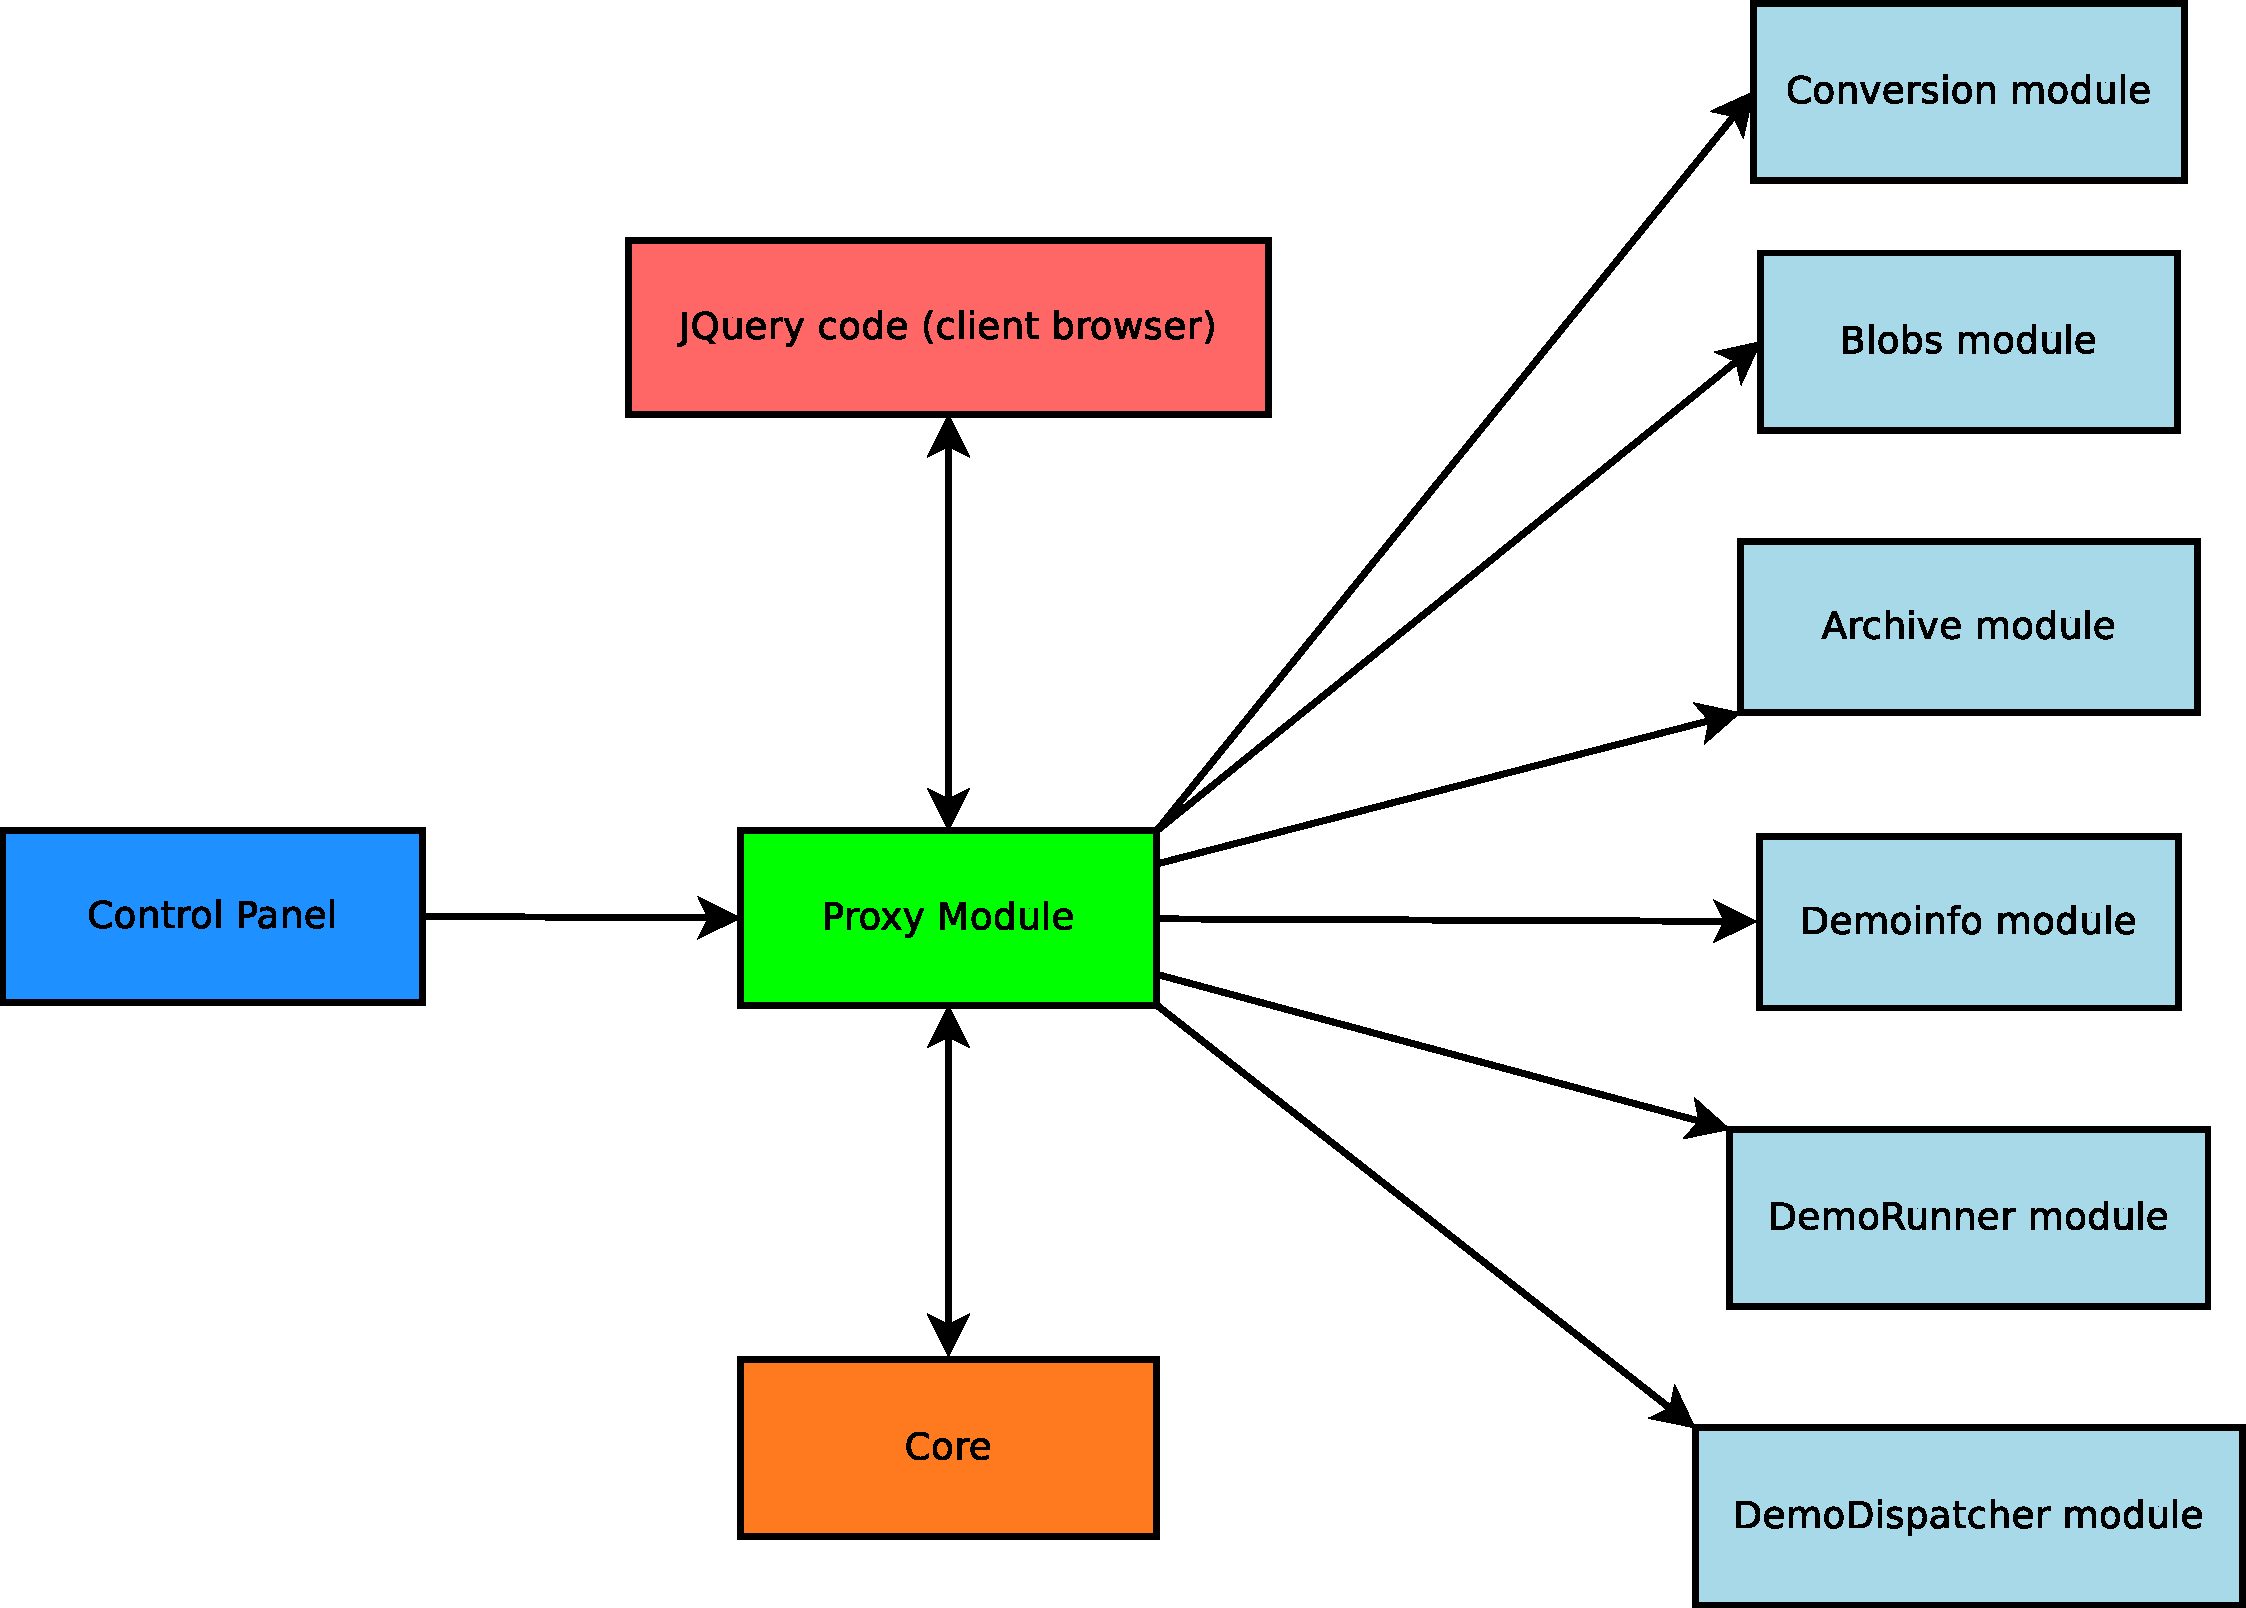
\includegraphics[width=0.8\linewidth]{architecture/images/architecture.pdf}
\caption{Modular system architecture.} 
\label{fig:architecture}
\end{figure}


% Project management and development methodology
% Project management and development methodology

\section{Project management and development methodology}
\miguel{For the moment this section is just a stub. Writing needed.}

\subsection{Project management}

\begin{itemize}
  \item We use CI
  \item Only commit when totally finished
  \item Trello
  \item Slack
\end{itemize}

\subsection{Development methodology}

\ToDo{Explain Continuous Integration, and the integration and production server}

Design Patterns \cite{GoF}, refactoring \cite{fowler1999refactoring}.

There are two git branches:

\begin{itemize}
  \item \textbf{master}: development
  \item \textbf{prod}: production
\end{itemize}

The {\tt master} branch is the default, where all development contributions are made. The testing server is configured to fetch this branch.

The {\tt prod} branch is for production. It is merged with {\tt master} only when the master is stable and one wants to integrate the changes in production. The production servers fetch this branch.

The {\tt prod} branch was created with:
\begin{verbatim}
git checkout -b prod
git push --set-upstream origin prod
\end{verbatim}

The .git/config ends up as:

\begin{verbatim}
[core]
	repositoryformatversion = 0
	filemode = true
	bare = false
	logallrefupdates = true
[remote "origin"]
	url = git@github.com:mcolom/ipolDevel.git
	fetch = +refs/heads/*:refs/remotes/origin/*
[branch "master"]
	remote = origin
	merge = refs/heads/master
[branch "prod"]
	remote = origin
	merge = refs/heads/prod
\end{verbatim}

To merge {\tt prod} with {\tt master:}
\begin{verbatim}
git checkout prod
git merge master
git push
git checkout master
\end{verbatim}



% The Core module
\section{The Demo System Core}
\ToDo{
OLD text. 
Centralized webservice.
The list of datatypes used (images, audio, video, 3D pointclouds, 3D meshes) and how to identify them. The "no type" format for demos which have their own non-standard format.}

In this section we explain the demo system core, that is the responsible of the coordination of the other modules. One of its main issues is controlling the execution of the different experiments. Figure \ref{fig:core_diagram} shows a diagram that explains the modules and the messages passed when executing an experiment.

The core performs very simple actions like creating the directories, copy the blobs for the experiment, etc, for ensuring that everything is ready for a demo execution. It delegates in the Demo Dispatcher module (see Sect.\ref{sec:DemoDispatcher}) the selection of the computer for the experiment. 

In order to distribute the load in several machines, this module checks the work load of each known DemoRunner modules (see Sect.~\ref{sec:DemoRunner}) and starts an algorithm demo execution on the less loaded machine. It uses a FIFO queue as a ``buffer'' to wait for a computer free to execute the demo and encapsulates an object to establishes the balancing policy that decides whether a process can leave the queue or not. Finally, the core uses the selected machine and waits until the experiment is finished. When it is finished, the core send to the archive module (see Sect.~\ref{sec:archive}) a JSON message for storing the experiment information.


\begin{figure}[!ht]
\centering
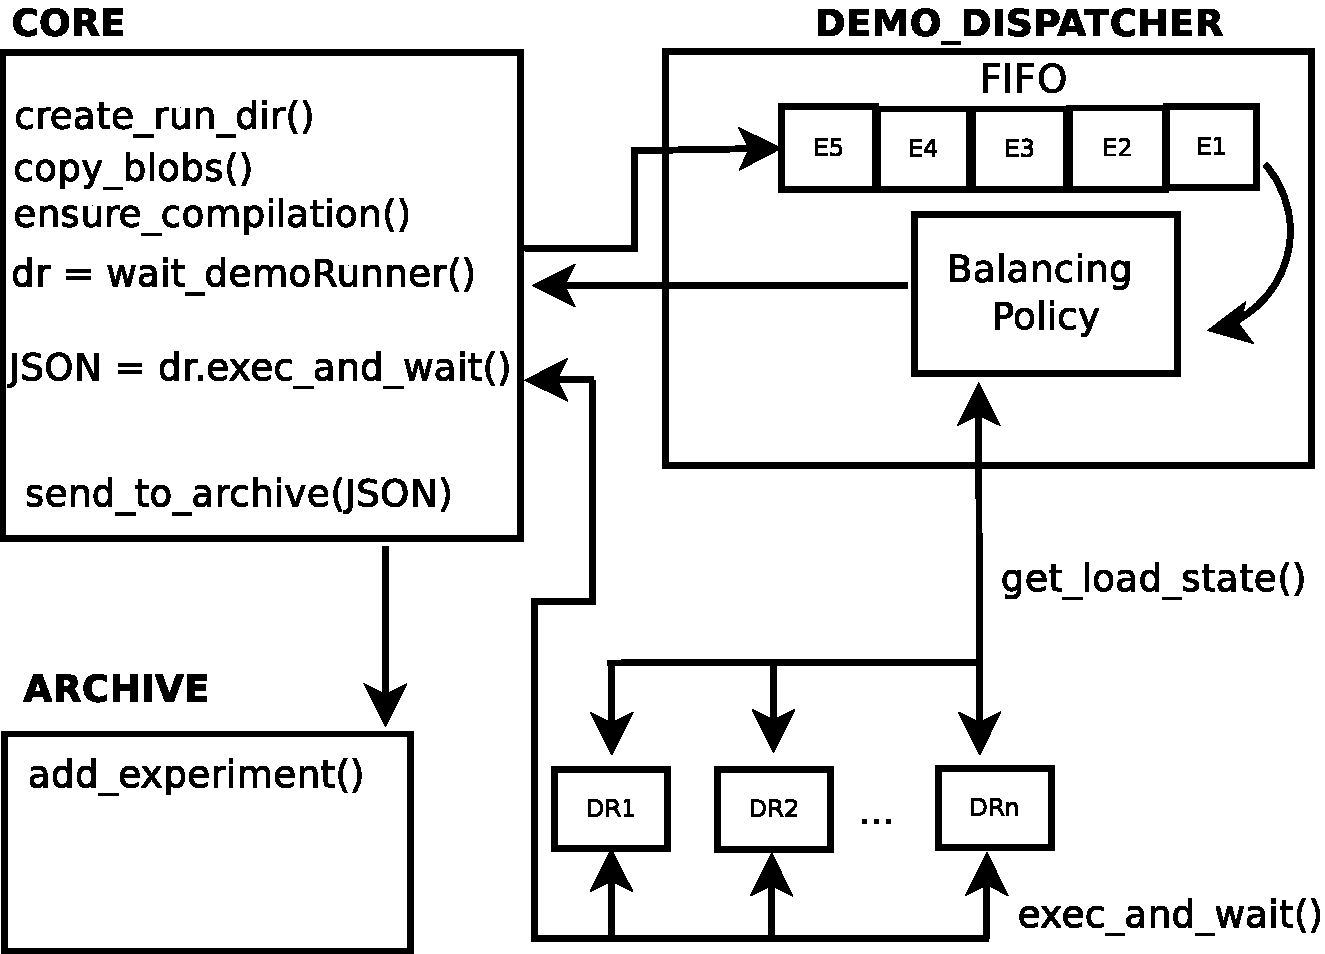
\includegraphics[width=0.7\columnwidth]{core/images/core_diagram.pdf}
\caption{Representation of the IPOL demos execution system.} 
\label{fig:core_diagram}
\end{figure}


\ToDo{Document it!}


% The Blobs module
\section{The Blobs module}

Note: to avoid confusion, we refer the modules of the IPOL system as ``ipol modules'' and Python modules (files containing Python code) as ``Python modules''.

\subsection{Introduction}
Each demo of IPOL offers the user a set of defaults blobs. Thus, the users are not forced to supply their own files for the executions of the algorithms. These defaults blobs can be tagged and linked to differents demos.

\subsection{Composition}
The blobs module is composed of several Python modules. It is composed of the same technical stack as the rest of the rest of the IPOL modules: written in Python, using a web server, a database, and using templates for generating HTML responses for webservices destinated to humans.

\subsubsection{Main Python module}
The main module is called by ``start.sh'', the script called by the control terminal to get modules running on different servers over ssh. It consist of setting up some variables used by cherrypy, as well as mounting the blobs class at the root of the used server.

\subsubsection{Error Python module}
This module describes the errors issued by the Blobs IPOL module and adds color to the error messages printed in the terminal.

\subsubsection{Database and database Python module}
The first and most important design constraint of the Blobs IPOL module was that data shouldn't be duplicated. All blobs referenced by multiple demos should exist in only one directory. This is addressed by establishment of one relational database, referencing the demos, the blobs, and the relationship between them. This database also permits to tag some text on blobs, as well as organize them in named sets. In the big picture, the database Python module a implement a simple CRUD\footnote{Acronym for Create, Read, Update, Delete. These operations allows the total manipulation and the persistancy of data inside a data structure.} interface for manipulating the database. Blobs can be managed individually, and upon the deletion of a demo, the blobs related to this demo will be deleted from disk if and only if they were uniquely linked to this demo. Blobs are referenced via their hashes, making it easy to verify if a blob is already in the database, even under another filename. \\

\begin{figure}[h]
\centering
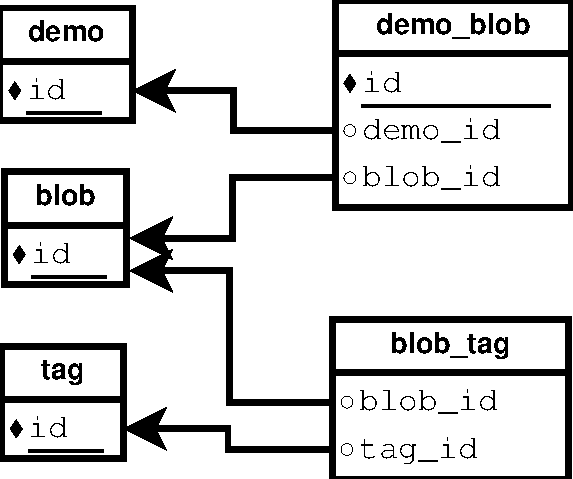
\includegraphics[scale=0.75]{blobs/images/blobs_database.pdf}
\caption{The database architecture of the blobs module} 
\label{fig:blobs_database}
\end{figure}


In the figure~\ref{fig:blobs_database}, id fields are the primary keys (it is worth noting that the primary key of a blob\_tag entry is the combination of the foreign keys it contains), the other fields are foreign keys, and the arrows indicate which primary keys are referenced by which foreign keys.
Three tables, demo, blob and tag, contains the information about referenced demos, blobs, and tags relating to blobs. Two junction tables link this information together, referencing the blobs standards to a demo, and the tags owned by each blobs.

\paragraph{The database Python module\\}
This module offers an interface for accessing the database. One object of the class Database should be instanciated for each operation modifying it. Even if it has function for connecting and closing, they should not be used as such, for flow control issues (for example, an exception leaving a connection open). A very simple abstraction, the DatabaseConnection class is present in the blobs Python module for it, and allow safe connection to the database, ensuring they will always be closed no matter what.

Otherwise, this Python module offer us a wide variety of simple methods for interacting with the database, or obtaining metrics of it, such as the total number of blobs. They generally return the information asked if such case apply. For the format of the responses and the different function, we refer the reader to the code of the module itself. It is worth noting that one webservice, delete\_blob\_from\_demo, recompute the positions of the blobs in a set in which a blob was deleted. If this function is accessed concurrently by multiple threads (the most likely case is if a webservice calling this function is accessed several times in a very short span), the blobs can end up with miscalculated positions. Non-concurrential access should be enforced by locking the scope where this webservice is called. Such a lock is used in the delete\_blob\_ws webservice in the blobs Python module.

\subsubsection{Blobs module}
The blobs Python module is the core of this. It implement three classes, DatabaseConnection as referenced earlier in the present documentation, and MyFieldStorage, for intermediate storage of the uploaded blobs in the /tmp/ directory, and Blobs as an encapsulation of the webservices and the data they use. It also has some utilitary function.

The Blobs class implements all the webservices constituting this module, both those transmitting JSON to other modules, and those generating HTML via templates for humans. An instance of the Blobs class should possess information about the storage of blobs and the networking parameters cherrypy use, such as a port number. A cherrypy configuration file, named ``blobs.conf'' contains the informations one might need to change to run the module on another server, without changing the code, such as the directories where the blobs can be found, the port used by the cherrypy engine, or the path to the database.

The webservices of the module access the database via instanciations of Database objects managed by the DatabaseConnection class. Some read information, and some modify the database by adding or removing information. For handling a webservice automatically and charging his JSON response as a Python object, the utilitary function use\_web\_service is used.

Logging is utilized as a mean to retrieve the errors occuring in the system. The logger implemented in the blobs Python module handle all the errors of the module. It is passed to each Database object instanciation.

Here is a list of all the webservices implemented by the blobs module :

\begin{itemize}
\item default : The service invoked when asked for non-existing service.
\item index : web page at the root of where the module is mounted in cherrypy.
\item blob : web page used to upload one blob to one demo.
\item archive : Used to upload one zip file of compressed blobs to one demo.
\item add\_blob\_ws : service checking that the given blobs do not exist in the database. If this is the case, add it.
\item add\_blob : implement the add\_blob page.
\item demos\_ws : return the list of demos from the database.
\item get\_template\_demos\_ws : return the list of template demos from the database
\item demos : web page used to add a demo to the database.
\item set\_template\_ws : webservice used to change the template used by a demo.
\item use\_template : web page used to change the template used by a demo.
\item add\_demo\_ws : web service used to add a demo to the database.
\item add\_demo : web page used to add a demo to the database.
\item add\_from\_archive : webservice used to upload a zip file of compressed blobs to one demo.
\item add\_tag\_to\_blob\_ws : webservice used to add a tag to a blob.
\item op\_add\_tag\_to\_blob : web page used to add a tag to a blob.
\item remove\_tag\_to\_blob\_ws : webservice used to remove a tag from a blob.
\item op\_remove\_tag\_to\_blob : web page used to remove a tag from a blob.
\item op\_remove\_blob\_from\_demo : web page used to remove a blob from a demo.
\item get\_blobs\_from\_template\_ws : webservice used to get the list of blobs from templated demo.
\item get\_blobs\_of\_demo\_by\_name\_ws : webservice returning a list of the hashes of the blobs owned by given demo name.
\item get\_blobs\_of\_demo\_ws : same as the precedent, but with the demo id.
\item get\_blobs\_of\_demo : web page used to display blobs owned by a given demo.
\item edit\_blob : web page showing the thumbnail of a demo with the possibility to add or remove tags.
\item get\_blob\_ws : webservice returning information about a blob from its id.
\item get\_tags\_ws : webservice returning tags of a blob from its id.
\item op\_remove\_demo\_ws : webservice removing a demo from its id.
\item op\_remove\_demo : web page used for removing a demo.
\item ping : used by the terminal for checking module status.
\item shutdown : used by the terminal for turning off the module at distance.
  
\end{itemize}


% The Archive module
\section{The Archive module}

\subsection{Introduction}
\label{sec:archive_introduction}

%\paragraph{Introduction} \hspace{0pt} \\
The archive module is a standalone application destinated to communicate with other modules using webservices. It is designed to implement a stable, simple and scalable system for archiving all experiments done with IPOL.

\paragraph{Technologies used} \hspace{0pt} \\
The archive module is written in Python, is using the cherrypy framework for webservices, the mako template library for webpage rendering, the Python Image Library for thumbnails creations, and the python-magic library available on pip (not to be mistaken with python-magic5 which is the one available on default ubuntu's APT repositories). The module communicate using JSON, both in input and output. The database engine used is SQLite.

\subsection{Architecture}

\paragraph{Module composition} \hspace{0pt} \\
The module is composed of very few files, the code itself in ``module.py'', a cherrypy configuration file ``archive.conf'', two mako HTML templates, and a database. It will also need 4 directories, respectively for storing blobs, thumbnails, the database and logs.

\paragraph{Module architecture} \hspace{0pt} \\
The module is composed of a class, Archive, encapsulating the datas needed to function. The services offered by the module are all methods of this class. The cherrypy framework provide the abstraction for making available the methods as webservices. \\
Upon starting the module, the cherrypy engine is launched, an object of the Archive class is created, and the cherrypy configuration is loaded from ``archive.conf''. If they don't exists, both the database and the directories needed for the storage of blobs, logs, the database and thumbnails will be created, provided that the user launching the module has the necessary rights. Otherwise, the module will not start. These directories are indicated in the cherrypy configuration for maximum configurability, if they are missing from it, the module will not start. \\
The webservices communicate with the server via arguments given through URL, as unicode strings directly passed to the methods. \\
The services all connect to the database in a thread-safe way, instanciating its own connection when called, commiting when done if there is modifications, or rollbacking if there is an error, and closing the connection. \\
There is a logger initialised with the Archive object, writing errors in ``error.log'' in the logs directory given in the configuration file.

\subsection{Database design}

The database contains 3 tables : experiments, blobs, and correspondence.\\
Each experiments, and each blobs are defined individually, and linked to each-others in the correspondence table, assuring a many-to-many connection. It is worth noting that the database doesn't save duplicates of the same blob. \\

\begin{tabular}{|l|c|r|}
  \hline
  experiments & blobs & correspondence \\
  \hline
  id & id & id \\
  id\_demo & hash & id\_experiment \\
  params & type & id\_blob \\
  timestamp & format & name \\
  \hline
\end{tabular} \\

\paragraph{Experiments table} \hspace{0pt} \\
The experiments table is defined as such : the id field, that store the unique id of the experiment ; the id\_demo field, that store the id of the IPOL demo used for the experiment ; the params field, which is a JSON string whose format vary from demo to demo ; and finally the timestamp field.

\paragraph{Blobs table} \hspace{0pt} \\
The blobs table is defined as such : the id field, that store the unique id of the blob ; the hash field, that store the hash of the blob computed with sha1, the type field, that store the extension of the blob (exemple ``jpeg'' or ``png''), and the format field, that store the media format of the blob : it is a string, either ``audio'', ``video'' or ``image''. \\
The physical location of a blob is ``blob\_dir defined in configuration file'' + ``hash of the blob'' + ``.'' + ``type of the blob''.

\paragraph{Correspondence table} \hspace{0pt} \\
The correspondence table is defined as such : the id field ; the id of the experiment and the id of the blob that is linked to said experiment, and the name field, which indicate the role of the blob in the experiment (example : ``input'' or ``denoised''). A foreign key constraint allowing cascade delete is put on the field id\_experiment, referencing the id of an entry in the experiment table, for automatic data deletion.

\subsection{Services}

\paragraph{Adding an experiment to the archive} \hspace{0pt} \\
The method ``add\_experiment'' take in entry the id of the demo used ; a JSON string of the format : 

\begin{tabbing}
tabs \= tabs \kill
\{ \\
\>url\_blob : name\}, \\
\> ... \\
\} \\
\end{tabbing}

containing a description of each blobs used by and produced by the experiment, with their temporary URLs and names ; and a JSON string describing the parameters of the demo used for the experiment. It will add an experiment to the database by creating a new entry in the experiment table. If the blobs used by and produced by the experiment aren't already in the database, it will copy them in the directory given in the configuration file, and, for the images, create a thumbnail. It will return a json string containing the status of the operation, OK uf it succeeded, KO if there was an error and the operation wasn't performed, as such :

\begin{tabbing}
tabs \= tabs \kill
\{ \\
\>status : OK/KO\}, \\
\} \\
\end{tabbing}

If status is KO, a log describing the error will be written.

\paragraph{Deleting an experiment from the archive} \hspace{0pt} \\
When removing an experiment from the database via the method ``delete\_experiment'', every blobs linked to this experiment and only to this experiment are removed. After that, all the entries in the correspondence table referencing this experiment are removed automatically due to a foreign key constraint. It return a json response containing the status of the operation of the same format as the return of the method ``add\_experiment''.

\paragraph{Deleting a blob from the archive} \hspace{0pt} \\
Due to a many-to-many link between blobs and experiments in the database, a blob has a lot of dependencies : it has of course the experiments using this blobs, but also the blobs linked to these experiments. For deleting a blob from the archive, the precedent service is called on each experiment the blob is part of, assuring that no orphans datas stay in the database (for exemple, experiments linked to removed blobs or blobs linked to removed experiments). The method implementing this service is ``delete\_blob\_w\_deps''. It return a json response containing the status of the operation of the same format as the return of the method ``add\_experiment''.

\paragraph{Getting datas from an archive page} \hspace{0pt} \\
The method ``page'' return in a JSON response, for a given page of a given demo, all the datas of the experiments that should be displayed on this page. Twelve experiments are displayed by page. For rendering the archive page in the browser, the JSON response should be parsed and interpreted in a dedicated template furnished by the front-end of another module. The JSON response is formatted this way : 
\begin{tabbing}
tabs \= tabs \= tabs \= tabs \= tabs \= tabs \kill
\{ \\
\> status :  OK/KO, \\
\> experiments : [ \\
\> \> \{ \\
\> \> \> date : timestamp\_example, \\ 
\> \> \> files : [ \\
\> \> \> \>  \{ \\
\> \> \> \> \> url : url\_example, \\
\> \> \> \> \> id : id\_example, \\
\> \> \> \> \> name : name\_example, \\
\> \> \> \> \> url\_thumb : url\_thumbnail\_example \\
\> \> \> \> \} \\
\> \> \> ... ], \\
\> \> \> id : id\_example, \\
\> \> \> parameters = \{parameters\_example...\} \\
\> ... ], \\
\> id\_demo : id\_demo\_example, \\
\> nb\_pages : nb\_pages\_example \\
\} \\
\end{tabbing} 

\paragraph{User interface for removing blobs/experiments} \hspace{0pt} \\
The only user interface furnished by the archive module is for removing blobs or experiment in a convenient manner. It use the json response of the precedent service and render the ``archive\_admin\_tmp.html'' template displaying a page of archive for given demo, allowing the deletion of both blobs and experiments by simply linking to two other services calling deletion methods and updating the template. In case of error, for example when invalid datas are given through URL, ``error.html'' is rendered.

\paragraph{Shutdown} \hspace{0pt} \\
The method ``Shutdown'' shutdown the archive application when called. It return a json response containing the status of the operation.

\paragraph{Other services}
Other services features the method ``ping'', simply for checking if the module is up, and the method ``stats'', formatted this way :
\begin{tabbing}
tabs \= tabs \kill
\{ \\
\> status : OK/KO, \\
\> nb\_experiments : x, \\
\> nb\_blobs : y \\
\} \\
\end{tabbing}


% The Demo Info module
\section{DemoInfo module}
This module store the textual description of the demo and allows to ask for specific sections of it. It also stores other demo-related information, as:
\begin{itemize}
\item Demo id
\item Abstract
\item Title 
\item Autors list
\item Autors email list
\item Article URL
\item State (inactive,preprint, published)
\item Demo editor
\item Demo editor email
\item Demo zip file containing demo DDL 
\item Demo DDL Json
\end{itemize}

This module will be used by the controll panel module, the demo will be extracted from the zip file, it will be created in Demoinfo module, The blobs will be addede to Blobs module.

\subsection{ demoinfo module structure}
This Module is formed by:
\begin{itemize}
\item model.py where the db structure, the DAO (Data access object) clasess and some helper claseses (Demo, Authorand Editor) are defined. It provides a layer of abstarction over the DB.
\item demoinfo.conf it's the cherrypy config for the webservices module.
\item demoinfo.py it's the webservices module.
\item testdemoinfo.py it's the tests to chech that the webservices work.
\item testdemoinfo.conf it's the cherrypy config for testing.
\end{itemize}

\subsection{The model (database) structure}
The model of this module id formed by the following tables:

\begin{figure}[!ht]
\centering
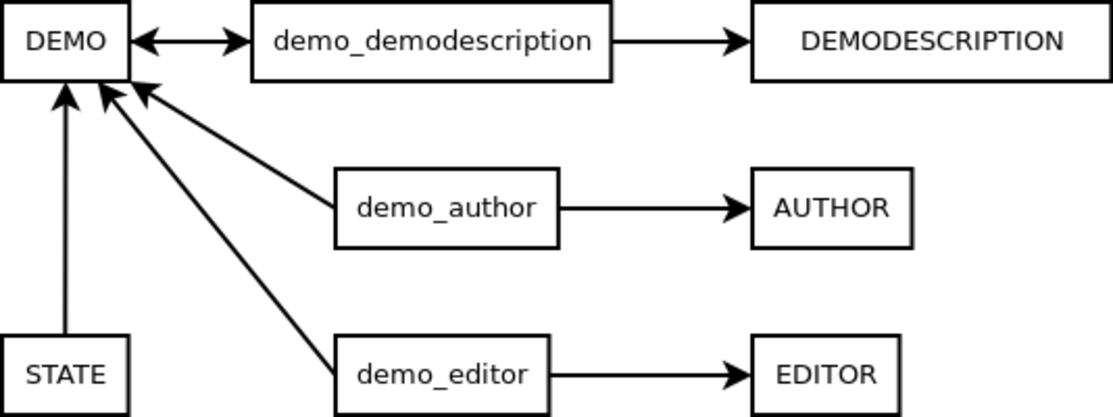
\includegraphics[width=0.5\columnwidth]{demo_info/images/demoinfo_model.pdf}
\caption{Demoinfo Database Model.} 
\label{fig:demoinfo_model}
\end{figure}

Note that states is the table for the demo's state (Published,preprint...)
Demodescription table is where the demo description language (DDL) for each demo is stored.
A demo may be created without a DDL (but you will need to provide one so you can run it)
Ddlschema is not used at the moment, but it has been created so that a schema validation can be done to the DDL of each demo, if a user provides a valid json for the DDL but this json is not a valid DDL , whe should be able to detect thisand return an error.

\subsection{Web services available}
This module provides a set of webservices, those that return data can be called with GET or other html methods, those that delete,create or update data can be called only by POST.
These webservices are shown grouped by functionality, 


DEMO

\begin{itemize}
\item  demo\_list(self)
\item  demo\_list\_by\_demoeditorid(self,demoeditorid\_list)
\item  demo\_list\_pagination\_and\_filter(self,num\_elements\_page,page,qfilter=None)
\item  demo\_get\_authors\_list(self,demo\_id)
\item  demo\_get\_available\_authors\_list(self,demo\_id)
\item  demo\_get\_editors\_list(self,demo\_id)
\item  demo\_get\_available\_editors\_list(self,demo\_id)
\item  demo\_get\_demodescriptions\_list(self,demo\_id,returnjsons=None)
\item  read\_demo\_metainfo(self, demoid)
\item  read\_demo\_metainfo\_by\_editordemoid(self, editordemoid)
\item  add\_demo(self, editorsdemoid, title, abstract, zipURL, active, stateID, demodescriptionID=None, demodescriptionJson=None)

Allows you to create a demo
- allow only post
- only creating the demo
- creating the demo and assigning an existing ddl (with id demodescriptionID) to it
- create the demo and create a ddl , whith the json passed by param (demodescriptionJson)

\item  delete\_demo(self,demo\_id,hard\_delete = False)
allow only post
\item  update\_demo(self,demo)
allow only post
\end{itemize}


AUTHOR

\begin{itemize}
\item  author\_list(self)
\item  author\_list\_pagination\_and\_filter(self,num\_elements\_page,page,qfilter=None)
\item  read\_author(self, authorid)
\item  author\_get\_demos\_list(self,author\_id)
\item  add\_author(self,name, mail)
allow only post
\item  add\_author\_to\_demo(self,demo\_id ,author\_id)
allow only post
\item  remove\_author\_from\_demo(self,demo\_id ,author\_id)
allow only post
\item  remove\_author(self,author\_id)
allow only post
\item  update\_author(self,author)
allow only post
\end{itemize}


EDITOR

\begin{itemize}
\item  editor\_list(self)
\item  editor\_list\_pagination\_and\_filter(self,num\_elements\_page,page,qfilter=None)
\item  editor\_get\_demos\_list(self,editor\_id)
\item  read\_editor(self, editorid)
\item  add\_editor(self,name, mail)
allow only post
\item  add\_editor\_to\_demo(self,demo\_id ,editor\_id)
allow only post
\item  remove\_editor\_from\_demo(self,demo\_id ,editor\_id)
allow only post
\item  remove\_editor(self,editor\_id)
allow only post
\item  update\_editor(self,editor)
allow only post
\end{itemize}

DDL

\begin{itemize}
\item  read\_demo\_description(self, demodescriptionID)
\item  read\_last\_demodescription\_from\_demo(self,demo\_id,returnjsons=None)
\item  add\_demodescription\_to\_demo(self,demo\_id, demodescription\_id)
allow only post
\item  add\_demo\_description(self,demoid=None,inproduction=None)
allow only post
\item  add\_demo\_description\_using\_param(self, demojson,inproduction = None)
\item  update\_demo\_description(self, demodescriptionID)
\end{itemize}

MISCELLANEA

\begin{itemize}
\item  index(self)
\item  ping(self)
\item  shutdown(self)
\item  stats(self)
\item  read\_states(self)
\end{itemize}


\subsection{Module testing}
To test this module enter test folder and run 
\begin{lstlisting}[language=Python,firstnumber=1]
python -m unittest discover.
\end{lstlisting}

To perfom manual testing use curl or poster pluguin for firefox (remember that some will only work with post requests) but in testdemoinfo.py, in the last tests you will find a working example of how to use some webservices using the request python library.
If you add webservices, please add the corresponding tests.


% The Demo Dispatcher module
\section{Dispatcher module}
\label{sec:Dispatcher}
\subsection{Introduction}
In order to distribute the load in several machines, this module is responsible to assign a demorunner according to a policy and the given requirements. 
The demorunners list is provided by the core module wich is in charge of reading the demorunners.xml where all the demorunners are. If the 
demorunner.xml file changes, there are two ways for reload the list loaded in memory, the first one is calling the function refresh\_demorunners
in the core and the other one is reloading the core and dispatcher module.

\subsection{Policies}
The creation of the policies are made by the Factory Method, allowing the implementation and assignment of new policies in an easy way.
Until now the implemented policies are:

\begin{itemize}
\item \textbf{Random Policy:} this policy assigns a random demorunner from the available demorunners list that matches the requirements.
\item \textbf{Sequential Policy:} this policy iterates from the available demorunners list that matches the requirements.
\item \textbf{Lowest Workload Policy:} this policy assigns the demorunner with the lowest workload from the available demorunners list that matches the requirements.
\end{itemize}


% The Demo Runner module

\section{DemoRunner module}
\label{sec:DemoRunner}

This module controls the execution of the IPOL demos. It can execute directly its binaries or supporting scripts (provided by the demo editors) related to a particular demo (demoextras). Besides, a demo editor can use some generic scripts (PythonTools) that helps for representing the results of a demo such as draw 2D curves, draw histograms, counting lines and similar.

The DemoRunner intervines twice during an execution. First, this module is responsible of informing the Core about the load of the machine where it is running and ensuring that the demo execution is done with the last source codes provided by the authors (it downloads and compiles these codes to maintain them updated). Second, the Demorunner executes the algorithm with the parameters set by the users. It takes care of stopping the demo execution if a timeout is reached, and to inform the Core about the causes of a demo execution failure so the Core can take the best action in response. 

% The Control Terminal 
\section{The Control Terminal}

\subsection{Introduction}
The Control Terminal is a small application intended to system administrators which allows to start, stop, and query the status of each module. It is composed of an XML file describing each modules, and of the terminal itself, a python script. \\
Upon launch, a prompt will appear, asking the user for a command.

\subsection{Architecture}
The terminal allows the user to type a variety of commands, for controlling the states of each modules composing the IPOL system. Some take parameters, generally the name of a modules. Every command is coded in the terminal script, and the XML file list for every module, the commands that can be used with this module as parameter.

\paragraph{XML file} \hspace{0pt} \\
The XML file ``modules.XML'' is parsed at the beginning of the execution of the python terminal for storing a dictionnary describing each module. \\
For security purposes, it is important to stress that the IPOL system must be deployed in a way of making this file trusted input : a call to the system() function in the terminal using content of this file open the way to a shell remote exploit if someone were to modify it. \\
Each module is defined by the attribute ``name'' and contain a variable number of tags : ``url'', ``server'', and ``path'', each describing respectively the url where the services provided by the module can be accessed, the server where the module is, and the path to the modules directory on said server. After that, an undefined number of ``command'' tags allow the module to be given as parameter for said commands. In order to function, the commands start, ping and shutdown.

\paragraph{Structure of the dictionnary parsed from the XML file} \hspace{0pt} \\
The dictionnary has, as keys, the name of each modules, and as value, another dictionnary with the following keys : ``url'', ``server'', ``path'', ``commands''. All of them but ``commands'' take as value the strings in the XML file server. The last key, ``commands'', takes as value a list of strings, each being a command available to the module. This list contains every string in ``command'' tags in the XML file, plus the string ``info'', which is added automatically. This dictionnary is the only attribute of the terminal object, initiated as ``self.dict\_modules''.

\paragraph{Execution loop} \hspace{0pt} \\

Upon start of the terminal, a ``Terminal'' object is created, the XML file is parsed as described before, then the data is stocked in a dictionnary, as the state of the ``Terminal'' object. This state should not change during the execution. After that, a simple loop is iniated, asking the user for input, evaluating said input and printing the result. For parsing the input, an entry buffer is used, with as key, the strings corresponding to the commands, and as value, the function executing said command (one could argue, the command itself). The input string is split in a list of words, the separation character being the space or `` ``. Then, the first word is given to the entry buffer for determining the function the user want to call, and the rest of the list is passed as parameter, allowing the retrieval of the parameters in the commands functions. \\
The loop repeat until an EOF indicator is encountered or if the input string is ``exit''. As such, ``exit'' is not a command, and no call to the exit syscall are being made, not allowing for exiting with a given value. \\
The terminal doesnt possess features such as pipes, redirections and multiples commands given in one input.

\subsection{Commands}

\paragraph{start} \hspace{0pt} \\
Usage :
\begin{verbatim}
start <module>
\end{verbatim}
The ``start'' command tale a module as parameter, ssh into the server where the module is located, and launch the module using its file start.sh. The command ``ping'' should be launched after for checking if the module is up.

\paragraph{ping} \hspace{0pt} \\
Usage :
\begin{verbatim}
ping <module>
\end{verbatim}
The ``ping'' command take a module as parameter, and call a webservice for checking if the module is up.

\paragraph{shutdown} \hspace{0pt} \\
Usage :
\begin{verbatim}
shutdown <module>
\end{verbatim}
The ``shutdown'' command take a module as parameter, and call the webservice for this module to shutdown.

\paragraph{info} \hspace{0pt} \\
Usage :
\begin{verbatim}
info <module>
\end{verbatim}
The ``info'' command take a module as parameter, and print the list of available commands for this module.

\paragraph{modules} \hspace{0pt} \\
Usage :
\begin{verbatim}
modules
\end{verbatim}
The ``modules'' command display a list of the modules.

\paragraph{help} \hspace{0pt} \\
Usage :
\begin{verbatim}
help
\end{verbatim}
The ``help'' command print the help of the terminal.


% The Access Control 
\section{Access control}
\label{sec:Access_control}
\subsection{Introduction}
To avoid the execution of exposed methods that allow the modification of the database (write and delete actions) by an unauthorized 
client, it has been created a wrapper that controls the access to these methods.

This wrapper compares the IP of the client that is calling the method with a list of authorized patterns. If the IP is authorized, 
the wrapper will automatically invoke the method requested by the client. Otherwise the request will be denied and the wrapper will 
respond with an Authentication Failed message.


\subsection{Authorized IPs File}
The file with the authorized IPs patterns is authorized\_pattern.conf, in the config\_common directory. This file consists
of a general section [Patterns], where all the permitted patterns are given with the following format: ``name=pattern''. Each pattern
allows the access of multiple IPs. 

The syntax for the pattern uses the asterisk to mean ``any''. For example: {\tt``local = 127.*.*.*''}

\subsection{Usage}
To add the authentication requisite to a method it is enough to add the {\tt@authenticate} decorator. It is important to add it 
below the {\tt@cherrypy.expose} decorator. Otherwise the method will not be longer exposed.


% Tools
\section{Tools}
This section describes the tools available for system administrators, developers, and editors to interact with the IPOL system. Some of their capabilities might clash with the Control Panel (for example, reading and modifying the DDL of the demos in the case of the DDL tool, Sec. \ref{sec:ddl_tool}), but they are useful to perform massive changes or to automatize tasks.

\section{The Control Terminal}

\subsection{Introduction}
The Control Terminal is a small application intended to system administrators which allows to start, stop, and query the status of each module. It is composed of an XML file describing each modules, and of the terminal itself, a python script. \\
Upon launch, a prompt will appear, asking the user for a command.

\subsection{Architecture}
The terminal allows the user to type a variety of commands, for controlling the states of each modules composing the IPOL system. Some take parameters, generally the name of a modules. Every command is coded in the terminal script, and the XML file list for every module, the commands that can be used with this module as parameter.

\paragraph{XML file} \hspace{0pt} \\
The XML file ``modules.XML'' is parsed at the beginning of the execution of the python terminal for storing a dictionnary describing each module. \\
For security purposes, it is important to stress that the IPOL system must be deployed in a way of making this file trusted input : a call to the system() function in the terminal using content of this file open the way to a shell remote exploit if someone were to modify it. \\
Each module is defined by the attribute ``name'' and contain a variable number of tags : ``url'', ``server'', and ``path'', each describing respectively the url where the services provided by the module can be accessed, the server where the module is, and the path to the modules directory on said server. After that, an undefined number of ``command'' tags allow the module to be given as parameter for said commands. In order to function, the commands start, ping and shutdown.

\paragraph{Structure of the dictionnary parsed from the XML file} \hspace{0pt} \\
The dictionnary has, as keys, the name of each modules, and as value, another dictionnary with the following keys : ``url'', ``server'', ``path'', ``commands''. All of them but ``commands'' take as value the strings in the XML file server. The last key, ``commands'', takes as value a list of strings, each being a command available to the module. This list contains every string in ``command'' tags in the XML file, plus the string ``info'', which is added automatically. This dictionnary is the only attribute of the terminal object, initiated as ``self.dict\_modules''.

\paragraph{Execution loop} \hspace{0pt} \\

Upon start of the terminal, a ``Terminal'' object is created, the XML file is parsed as described before, then the data is stocked in a dictionnary, as the state of the ``Terminal'' object. This state should not change during the execution. After that, a simple loop is iniated, asking the user for input, evaluating said input and printing the result. For parsing the input, an entry buffer is used, with as key, the strings corresponding to the commands, and as value, the function executing said command (one could argue, the command itself). The input string is split in a list of words, the separation character being the space or `` ``. Then, the first word is given to the entry buffer for determining the function the user want to call, and the rest of the list is passed as parameter, allowing the retrieval of the parameters in the commands functions. \\
The loop repeat until an EOF indicator is encountered or if the input string is ``exit''. As such, ``exit'' is not a command, and no call to the exit syscall are being made, not allowing for exiting with a given value. \\
The terminal doesnt possess features such as pipes, redirections and multiples commands given in one input.

\subsection{Commands}

\paragraph{start} \hspace{0pt} \\
Usage :
\begin{verbatim}
start <module>
\end{verbatim}
The ``start'' command tale a module as parameter, ssh into the server where the module is located, and launch the module using its file start.sh. The command ``ping'' should be launched after for checking if the module is up.

\paragraph{ping} \hspace{0pt} \\
Usage :
\begin{verbatim}
ping <module>
\end{verbatim}
The ``ping'' command take a module as parameter, and call a webservice for checking if the module is up.

\paragraph{shutdown} \hspace{0pt} \\
Usage :
\begin{verbatim}
shutdown <module>
\end{verbatim}
The ``shutdown'' command take a module as parameter, and call the webservice for this module to shutdown.

\paragraph{info} \hspace{0pt} \\
Usage :
\begin{verbatim}
info <module>
\end{verbatim}
The ``info'' command take a module as parameter, and print the list of available commands for this module.

\paragraph{modules} \hspace{0pt} \\
Usage :
\begin{verbatim}
modules
\end{verbatim}
The ``modules'' command display a list of the modules.

\paragraph{help} \hspace{0pt} \\
Usage :
\begin{verbatim}
help
\end{verbatim}
The ``help'' command print the help of the terminal.

% Instructions to modify this document:
% * Remember to ALWAYS execute "git pull" BEFORE any commit you make!
% * Use the \ToDo{...} command to remark tasks which still need to be done. Add your name in the comment.
% * Use the \input{file.tex} command to split the document into several parts
% * Do not change the current LaTeX coding style to yours. The style and format should be homogeneous along sections.

% To convert .dia diagrams into PDF:
% 1) Create the diagram with dia
% 2) Export it as .eps
% 3) use epstopdf to convert to PDF
%
% Editing SVG files and exporting them to PDF with Inkscape is admitted too.
% Remember to keep a copy of the editable file (.dia or .svg files).


\documentclass[a4paper,12pt]{article}

\usepackage[utf8]{inputenc}
\usepackage{amsmath,graphicx}
\usepackage{bm}
\usepackage{amssymb}
\usepackage{algorithm}
\usepackage{algpseudocode}
\usepackage{subfigure}
\usepackage{ifpdf}
\usepackage[hyphens]{url}
\usepackage{color}
\usepackage[hidelinks]{hyperref}
\usepackage{multirow}
\usepackage{datetime}
\usepackage{comment}
\usepackage{float} % To put figures in their exact place with \begin{figure}[H]
\usepackage{longtable}
\usepackage{tabularx}
\usepackage{listings}
\usepackage{xcolor}
\usepackage{color}

\definecolor{mygreen}{rgb}{0,0.6,0}
\definecolor{mygray}{rgb}{0.5,0.5,0.5}
\definecolor{mymauve}{rgb}{0.58,0,0.82}

\lstset{ %
  language=HTML,                 % the language of the code
  backgroundcolor=\color{white},   % choose the background color; you must add \usepackage{color} or \usepackage{xcolor}
  basicstyle=\small,        % the size of the fonts that are used for the code
  breakatwhitespace=false,         % sets if automatic breaks should only happen at whitespace
  breaklines=true,                 % sets automatic line breaking
  captionpos=b,                    % sets the caption-position to bottom
  commentstyle=\color{mygreen},    % comment style
  deletekeywords={...},            % if you want to delete keywords from the given language
  escapeinside={\%*}{*)},          % if you want to add LaTeX within your code
  extendedchars=true,              % lets you use non-ASCII characters; for 8-bits encodings only, does not work with UTF-8
  frame=single,                    % adds a frame around the code
  keepspaces=true,                 % keeps spaces in text, useful for keeping indentation of code (possibly needs columns=flexible)
  keywordstyle=\color{blue},       % keyword style
  language=HTML,                 % the language of the code
  otherkeywords={*,...},           % if you want to add more keywords to the set
  numbers=left,                    % where to put the line-numbers; possible values are (none, left, right)
  numbersep=5pt,                   % how far the line-numbers are from the code
  numberstyle=\tiny\color{mygray}, % the style that is used for the line-numbers
  rulecolor=\color{black},         % if not set, the frame-color may be changed on line-breaks within not-black text (e.g. comments (green here))
  showspaces=false,                % show spaces everywhere adding particular underscores; it overrides 'showstringspaces'
  showstringspaces=false,          % underline spaces within strings only
  showtabs=false,                  % show tabs within strings adding particular underscores
  stepnumber=2,                    % the step between two line-numbers. If it's 1, each line will be numbered
  stringstyle=\color{mymauve},     % string literal style
  tabsize=2,                     % sets default tabsize to 2 spaces
  title=\lstname                   % show the filename of files included with \lstinputlisting; also try caption instead of title
}


\definecolor{lightgray}{rgb}{.9,.9,.9}
\definecolor{darkgray}{rgb}{.4,.4,.4}
\definecolor{purple}{rgb}{0.65, 0.12, 0.82}
\lstdefinelanguage{JavaScript}{
  keywords={break, case, catch, continue, debugger, default, delete, do, else, false, finally, for, function, if, in, instanceof, new, null, return, switch, this, throw, true, try, typeof, var, void, while, with},
  morecomment=[l]{//},
  morecomment=[s]{/*}{*/},
  morestring=[b]',
  morestring=[b]",
  ndkeywords={class, export, boolean, throw, implements, import, this},
  keywordstyle=\color{blue}\bfseries,
  ndkeywordstyle=\color{darkgray}\bfseries,
  identifierstyle=\color{black},
  commentstyle=\color{purple}\ttfamily,
  stringstyle=\color{red}\ttfamily,
  sensitive=true
}

\newcolumntype{L}[1]{>{\raggedright\arraybackslash}p{#1}}
\newcolumntype{C}[1]{>{\centering\arraybackslash}p{#1}}
\newcolumntype{R}[1]{>{\raggedleft\arraybackslash}p{#1}}


% Definitions and commands
\def \np{\vskip 0.25 cm}
\def \ap{\vskip 0.15 cm}

% JSON listing (see 
%  http://tex.stackexchange.com/questions/83085/how-to-improve-listings-display 
% -of- json-files)
\colorlet{punct}{red!60!black}
\definecolor{background}{HTML}{EEEEEE}
\definecolor{delim}{RGB}{20,105,176}
\colorlet{numb}{magenta!60!black}

\lstdefinelanguage{json}{
    basicstyle=\footnotesize\ttfamily,
    numbers=left,
    numberstyle=\scriptsize,
    stepnumber=1,
    numbersep=8pt,
    showstringspaces=false,
    breaklines=true,
    frame=lines,
    backgroundcolor=\color{background},
    literate=
     *{0}{{{\color{numb}0}}}{1}
      {1}{{{\color{numb}1}}}{1}
      {2}{{{\color{numb}2}}}{1}
      {3}{{{\color{numb}3}}}{1}
      {4}{{{\color{numb}4}}}{1}
      {5}{{{\color{numb}5}}}{1}
      {6}{{{\color{numb}6}}}{1}
      {7}{{{\color{numb}7}}}{1}
      {8}{{{\color{numb}8}}}{1}
      {9}{{{\color{numb}9}}}{1}
      {:}{{{\color{punct}{:}}}}{1}
      {,}{{{\color{punct}{,}}}}{1}
      {\{}{{{\color{delim}{\{}}}}{1}
      {\}}{{{\color{delim}{\}}}}}{1}
      {[}{{{\color{delim}{[}}}}{1}
      {]}{{{\color{delim}{]}}}}{1},
}


\newcommand{\ToDo}[1]{\textcolor{magenta}{\textbf{[ToDo]} \textbf{#1}}}
\newcommand{\miguel}[1]{\textcolor{magenta}{\textbf{[Miguel]} \textbf{#1}}}


\begin{document}


\begin{titlepage}

\begin{center}
\vspace*{-1in}

\vspace*{0.6in}
\begin{Large}
\textbf{The IPOL Data Description Lines (DDL)} \\
\end{Large}

\vspace*{0.6in}

\small{Compiled on \today\ at \currenttime}

\vspace*{0.6in}
\rule{80mm}{0.1mm}\\
\vspace*{0.1in}
\end{center}

\end{titlepage}

This document contains the technical documentation for the Demo Description Lines (DDL) for the IPOL Demo System 2.0 for the real-time demos generation from their textual description.

\vspace*{0.6in}

%\maketitle
\newpage

\tableofcontents
\newpage

%\listoffigures
%\newpage

% The Demo Description Lines (DDL) reference
\section{Introduction}
The Demo Description Lines (DDL) is an abstract syntax which allows
defining an IPOL demo. The description is 
written in JSON (JavaScript Object Notation) format. This language is
evolving to allow a maximum number of demos to be described without the
need to manually write HTML or Python code 
for a given demo. Each main key in the description file is described
in the following sections:
\begin{itemize}
  \item \textit{general}: general options (required);
  \item \textit{build}: download and compile the source code (required);
  \item \textit{inputs}: description of the different inputs  (required);
  \item \textit{params}: description of the parameters, for the param page (recommended);
  \item \textit{run}: commands to run the demo (required);
  \item \textit{config}: configuration, saving demo information (optional);
  \item \textit{archive}: description of files  what is saved in archive when inputs are uploaded (optional);
  \item \textit{results}: displaying the result page (required).
\end{itemize}

\vspace{1em}

JSON data for IPOL should be strictly valid. Most common mistakes:
\begin{itemize}
  \item ASCII, no letters with diacritics or accents like 'é' or '$\sigma$', use HTML entities for special characters (ex: \&eacute; \&sigma;);
  \item commas, requested separator between items in list or dictionary, forbidden at start or end of a collection.
\end{itemize}
The IPOL control panel provides a JSON editor with a simple validator. Most of the syntax errors are detected in real time
and reported by a graphic hint. The non ASCII characters are not detected by the client. 
Before to be applied, the JSON data are validated by the server, and may be not accepted.

%-------------------------------------------------------------------------------
\section{The \emph{general} section}
The general section describes global information about the demo.
It is a set of  (key,value) pairs, described in the following table.
Many keys are derived from the static variables of the previous 'app' Python class.\\
% 
\begin{longtable}{|>{\bf}L{\dimexpr 0.28\linewidth}|L{\dimexpr 
0.57\linewidth}|c|}
\hline
 \centering {key}     & \centering {\bf description} & {\bf req} 
\tabularnewline \hline \hline
 demo\_title         & demo title & yes\\ \hline
 input\_description  & description at the top of the input selection page, 
                      contains HTML as a single string or as an array of string
                      that will be concatenated and separated with spaces.
                     & yes \\ \hline
 param\_description  & description at the top of the para\-meters page,
                      contains HTML as a single string or as an array of string
                      that will be concatenated and separated with spaces.
                      & yes
                      \\ \hline
 xlink\_article     & defines the link to the article webpage & yes  \\ \hline
 crop\_maxsize      & limit allowed crop size in both width and height, the string
                      can contain a JavaScript expression which will be evaluated & no \\ \hline
 requirements 	    & specify the particular requirements needed for the execution of the demo separated by commas. e.g. Matlab. & no \\ \hline
 timeout 	    & specify the time in seconds to execute the algorithm. If the execution takes longer than the specified time 
		      the system kills the process.& no \\ \hline
\caption{Keys for the 'general' section ({\em req} means required).}
\end{longtable}

%-------------------------------------------------------------------------------
\section{The \emph{build} section}

The build section contains an array of build descriptions in the form
''[ \{...\}, \{...\}, ...] ''. For each description, an archive containing the 
source code is downloaded and compiled using either 'make','cmake' or 'script' features.
It has the following information:

\subsection{\emph{make} type}

\begin{longtable}{|>{\bf}L{\dimexpr 0.25\linewidth}|L{\dimexpr 0.6\linewidth}|c|}
\hline
\centering {key}     & \centering {\bf description} & {\bf req} \tabularnewline 
\hline \hline
 build\_type    & make & yes \\ \hline
 url        & full url link to download the demo source code & yes \\ \hline
 srcdir     & subdirectory from the extracted archive where the source code is 
            located & yes \\ \hline
 prepare\_make & shell command used to fix compilation errors of the source code,
                since the source code is steady & no  \\ \hline
 binaries   & list of binaries and their associated paths relative to the source 
            code path. In case of 'make' build type, the first path is the compilation
            path, where the make command is called, the second path is the binary
            path. You can run make without a binary name by setting the second
            path to a directory (it should end with '/' character), then all files 
            from this directory will be copied
            to the demo binary path. If the second path is a directory, give 
            a third value corresponding to one of the files to be copied, so that
            the system can check the file timestamp to decide if a rebuild is needed.
            & yes \\ \hline
 flags      & make command compilation flags & yes \\ \hline
 scripts    & list of scripts and their associated paths relative to the source 
            code path & no  \\ \hline
 post\_build & shell command to run after the build & no \\ \hline
\caption{Keys for the 'make' type.}
\end{longtable}

\paragraph{Example}:\\
\begin{lstlisting}[language=json,firstnumber=1]
"build": [ 
  {
    "build_type"    : "make",
    "url"           : "http://www.ipol.im/../phs_3.tar.gz", 
    "srcdir"        : "phs_3",
    "binaries"      : [ [".","horn_schunck_pyramidal"] ],
    "flags"         : "-j4"
  {
    "build_type"    : "make",
    "url"           : "http://www.ipol.im/../imscript_dec2011.tar.gz", 
    "srcdir"        : "imscript",
    "binaries"      : [ [".","bin/", "plambda"] ],
    "flags"          : "-j CFLAGS=-O3 IIOFLAGS='-lpng -lm'"
  }
]
\end{lstlisting}

\subsection{\emph{cmake} type}

\begin{longtable}{|>{\bf}L{\dimexpr 0.25\linewidth}|L{\dimexpr 0.6\linewidth}|c|}
\hline
\centering {key}     & \centering {\bf description} & {\bf req} \tabularnewline 
\hline \hline
 build\_type  & cmake & yes \\ \hline
 url          & same as make type & yes \\ \hline
 srcdir       & same as make type & yes \\ \hline
 prepare\_cmake & shell command used to fix compilation errors of the source code,
                since the source code is steady & no  \\ \hline
 cmake\_flags  & cmake flags for configuration ('Release' build type is 
                automatically set) & no  \\ \hline
 binaries     & same as make type & yes \\ \hline
 flags        & same as make type & yes \\ \hline
 scripts      & same as make type & no  \\ \hline
 post\_build  & same as make type & no \\ \hline
\caption{Keys for the 'cmake' type.}
\end{longtable}

\paragraph{Example}:\\
\begin{lstlisting}[language=json,firstnumber=1]
"build": [ { 
  "build_type" : "cmake",
  "url"        : "http://www.ipol.im/xxx/ldm_q1p.zip", 
  "srcdir"     : ".",
  "binaries"   : [ [".","lens_distortion_correction"] ],
  "flags"      : "OMP=1 -j4" } ]
\end{lstlisting}

\subsection{\emph{script} type}

\begin{longtable}{|>{\bf}L{\dimexpr 0.25\linewidth}|L{\dimexpr 0.6\linewidth}|c|}
\hline
\centering {key}     & \centering {\bf description} & {\bf req} \tabularnewline 
\hline \hline
 build\_type  & script & yes \\ \hline
 url          & same as make type & yes \\ \hline
 srcdir       & same as make type & yes \\ \hline
 scripts      & same as make type & no  \\ \hline
\caption{Keys for the 'script' type.}
\end{longtable}

\paragraph{Example}:\\
\begin{lstlisting}[language=json,firstnumber=1]
"build": [ { 
    "build_type": "script",
    "url": "http://151.80.24.28:8080/DemoSource/1000003/demo_scripts.tgz",
    "srcdir": "demo_scripts",
    "scripts": [ [ ".", "write_line_parameters.py" ] ]
  }
\end{lstlisting}


%-------------------------------------------------------------------------------
\section{The \emph{inputs} section}
The inputs section describes the characteristics of the input data for the algorithm.

\subsection{\emph{image} type}

\begin{longtable}{|>{\bf}L{\dimexpr 0.26\linewidth}|L{\dimexpr 0.59\linewidth}|c|}
\hline
\centering {key}     & \centering {\bf description} & {\bf req} \tabularnewline 
\hline \hline
 type         & image & yes \\ \hline
 description  & Short name or description of the input, it will used to display 
the input as the label inside the 'gallery' HTML display & no \\ \hline
 max\_pixels   &  Sets the maximal number of pixels of the input image, 
bigger images will be downsized, if 0 no resizing is done. 
Input can be a number or a simple arithmetic expression as a string that will be evaluated (ex: "1000*1000" = 1 Mpx).  & yes \\ \hline
 max\_weight   & Maximum weight (in bytes) of an input file, prevents uploading 
bigger files.
Input can be a number or a simple arithmetic expression as a string that will be evaluated (ex: "100*1024*1024"= 100 Mb). & no \\ \hline
 dtype        & Expected data type for image to process:
\vspace{-1em}
\begin{itemize}
  \setlength\itemsep{-0.5em}
  \item \textit{1x8i}: gray, unsigned integer 8 bits;
  \item \textit{3x8i}: color, RGB unsigned integer 8 bits;
  \item \textit{1x16i}: gray, unsigned integer 16 bits;
  \item \textit{3x16i}: color, RGB unsigned integer 16 bits.
\end{itemize} & yes \\ \hline
 ext          & input image expected extension (ie. file format) & yes \\ \hline
forbid\_preprocess         & Forbids any pre-processing of the input data by IPOL system. 
Submitted image is kept as-is.
Used by algorithms like noise-estimation or modification detection, where re-sampling will affect results. 
If a processing is needed, according to the expected properties upper, the user will be informed by a message.
& no \\ \hline
\caption{Keys for the 'image' type.}
\end{longtable}

%-------------------------------------------------------------------------------
\section{The \emph{params} section}
The params section describes the set of parameters needed by a demo, their 
constraints and their visual appearance. It is defined as an array of sets, 
where each set contains (key,value) pairs.


\subsection{ \emph{range} type}

The values of the range type are stored as numbers, so no double quotes are 
required around the values. The default value is stored with the 'values' field.

\begin{longtable}{|>{\bf}L{\dimexpr 0.15\linewidth}|L{\dimexpr 
0.7\linewidth}|c|}
\hline
 \centering {key}     & \centering {\bf description} & {\bf req} 
\tabularnewline \hline \hline
 type  & range       & yes \\ \hline
 visible  & evaluated Javascript boolean expression. It hides the parameter if
            evaluated to false (if undefined the parameter is visible)& no \\ \hline
 id     & parameter name in lowercase letters  & yes \\ \hline
 label  & name and/or description of the parameter, appears on the left side. & yes
                      \\ \hline
 comments & description of the parameter, appears on the right side. & no
                      \\ \hline
 values & set min,max,step and default values using the following key/value 
scheme \{ 'min':val, 'max':val, 'step':val, 'default':val \} & yes
                      \\ \hline
\caption{Keys for the 'range' type.}
\end{longtable}


\subsection{ \emph{selection\_collapsed} type}

The values of the selection are stored as strings, so we map each label with a 
string value. The default value is stored in a separate field.

\begin{longtable}{|>{\bf}L{\dimexpr 0.25\linewidth}|L{\dimexpr 
0.6\linewidth}|c|}
\hline
 \centering {key}     & \centering {\bf description} & {\bf req} 
\tabularnewline \hline \hline
 type  & selection\_collapsed    & yes \\ \hline
 visible  & Evaluated Javascript boolean expression which hides the parameter if
            evaluated to false (if undefined the parameter is visible)& no \\ \hline
 id     & parameter name in lowercase letters & yes \\ \hline
 label  & name and/or description of the parameter, appears on the left side. & yes
                      \\ \hline
 comments & description of the parameter, appears on the right side. & no
                      \\ \hline
 values & set of (key,value) pairs, where the key is the displayed text and the 
value a string representing the corresponding value, for example \{ 
'black':'0', '1\%':'0.01' \} & yes
                      \\ \hline
 default\_value & defines the default value for this parameter, should be one 
the values defined in 'values'. & yes \\ \hline
\caption{Keys for the 'selection\_collapsed' type.}
\end{longtable}

\subsection{ \emph{selection\_radio} type}

The values of the selection are stored as strings, so we map each label with a 
string value. The default value is stored in a separate field.
This type is similar to the selection collapsed type, but display the different
options using radio buttons.

\begin{longtable}{|>{\bf}L{\dimexpr 0.25\linewidth}|L{\dimexpr 
0.6\linewidth}|c|}
\hline
 \centering {key}     & \centering {\bf description} & {\bf req} 
\tabularnewline \hline \hline
 type     & selection\_radio    & yes \\ \hline
 visible  & Evaluated Javascript boolean expression which hides the parameter if
            evaluated to false (if undefined the parameter is visible)& no \\ \hline
 id       & parameter name in lowercase letters & yes \\ \hline
 label  & name and/or description of the parameter, appears on the left side. & yes
                      \\ \hline
 comments & description of the parameter, appears on the right side. & no
                      \\ \hline
 vertical & boolean, if true use vertical display, otherwise use horizontal
            display (default=false) & no \\ \hline
 values   & set of (key,value) pairs, where the key is the displayed text and the 
value a string representing the corresponding value, for example \{ 
'black':'0', '1\%':'0.01' \} & yes
                      \\ \hline
 default\_value & defines the default value for this parameter, should be one 
the values defined in 'values'. & yes \\ \hline
\caption{Keys for the 'selection\_radio' type.}
\end{longtable}

\subsection{ \emph{label} type}

The label  can be used as a title to separate groups of parameters.

\begin{longtable}{|>{\bf}L{\dimexpr 0.27\linewidth}|L{\dimexpr 
0.58\linewidth}|c|}
\hline
 \centering {key}     & \centering {\bf description} & {\bf req} 
\tabularnewline \hline \hline
 type  & label       & yes \\ \hline
 visible  & Evaluated Javascript boolean expression which hides the parameter if
            evaluated to false (if undefined the parameter is visible)& no \\ \hline
 label & HTML text to display, as a single string or as an array of strings& yes
                      \\ \hline
\caption{Common keys for the 'label' type.}
\end{longtable}


\subsection{ \emph{checkbox} type}

\begin{longtable}{|>{\bf}L{\dimexpr 0.27\linewidth}|L{\dimexpr 
0.58\linewidth}|c|}
\hline
 \centering {key}     & \centering {\bf description} & {\bf req} 
\tabularnewline \hline \hline
 type  & checkbox  & yes \\ \hline
 visible  & Evaluated Javascript boolean expression which hides the parameter if
            evaluated to false (if undefined the parameter is visible)& no \\ \hline
 label  & name and/or description of the parameter, appears on the left side. & yes
                      \\ \hline
 comments & description of the parameter, appears on the right side. & no
                      \\ \hline
 id         & parameter name in lowercase letters  & yes \\ \hline
 default\_value & boolean: True for checked & \\ \hline
\caption{Common keys for the 'checkbox' type.}
\end{longtable}

\subsection{ \emph{checkboxes} type}

\begin{longtable}{|>{\bf}L{\dimexpr 0.27\linewidth}|L{\dimexpr 
0.58\linewidth}|c|}
\hline
 \centering {key}     & \centering {\bf description} & {\bf req} 
\tabularnewline \hline \hline
 type  & checkboxes   & yes \\ \hline
 visible  & Evaluated Javascript boolean expression which hides the parameter if
            evaluated to false (if undefined the parameter is visible)& no \\ \hline
 label  & name and/or description of the parameter, appears on the left side. & yes
                      \\ \hline
 comments & description of the parameter, appears on the right side. & no
                      \\ \hline
 id         & parameter name in lowercase letters  & yes \\ \hline
 values     & list of dictionaries: [ {key:value, ...}, ... ]
            where key is the checkbox id and value is the text associated
            & yes \\ \hline
 default     & list of checkboxes that are checked by default  & yes \\ \hline
\caption{Common keys for the 'checkboxes' type.}
\end{longtable}


\subsection{ \emph{numeric} type}

This param allows just numeric input
\begin{longtable}{|>{\bf}L{\dimexpr 0.27\linewidth}|L{\dimexpr 
0.58\linewidth}|c|}
\hline
 \centering {key}     & \centering {\bf description} & {\bf req} 
\tabularnewline \hline \hline
 type       & numeric   & yes \\ \hline
 visible    & Evaluated Javascript boolean expression which hides the parameter
              if evaluated to false (if undefined the parameter is visible) & no \\ \hline
 label      & name and/or description of the parameter, appears on the left side. & yes \\ \hline
 comments   & description of the parameter, appears on the right side. & no  \\ \hline
 id         & parameter name in lowercase letters & yes \\ \hline
 values     & set min,max,step and default values using the following key/value scheme \{ 'min':val, 'max':val, 'default':val \} & no \\ \hline
\caption{Common keys for the 'checkboxes' type.}
\end{longtable}

\subsection{ \emph{text} type}

This param allows numeric and text input
\begin{longtable}{|>{\bf}L{\dimexpr 0.27\linewidth}|L{\dimexpr 
0.58\linewidth}|c|}
\hline
 \centering {key}     & \centering {\bf description} & {\bf req} 
\tabularnewline \hline \hline
 type       & text   & yes \\ \hline
 visible    & Evaluated Javascript boolean expression which hides the parameter
              if evaluated to false (if undefined the parameter is visible) & no \\ \hline
 label      & name and/or description of the parameter, appears on the left side. & yes \\ \hline
 id         & parameter name in lowercase letters & yes \\ \hline
 values     & set maxlength and default values using the following key/value scheme \{ 'maxlength':val, 'default':val \} & no \\ \hline
\caption{Common keys for the 'checkboxes' type.}
\end{longtable}

%-------------------------------------------------------------------------------
\section{The \emph{params\_layout} section}

The default layout of parameters is to stack them together within an 'HTML field'
entitle 'Parameters:'. However, if a demo needs to group together some parameters,
it can use a specific params\_layout section that contains an array of
sets of parameters, where each set is defined by an array containing the group 
title as the first element and the list of parameters ids as the second element,
where the parameters ids are their position in the params section (starting at 0).

\paragraph{Examples}:\\
\begin{lstlisting}[language=json,firstnumber=1]
  "params_layout": [
        [ "General parameters:",          [ 0,1]  ],
        [ "Sampled Gaussian kernel",      [2]     ],
        [ "Lindeberg's smoothing method", [3]     ]
    ],
\end{lstlisting}

%-------------------------------------------------------------------------------
\section{The \emph{run} section}

The 'run' section contains an array of elements, where each element can be 
a string or another array of strings:
\begin{itemize}
\item if the element is a string starting with '\#', it is considered as a comment.
\item if the element is a string, it can be a command to run from the system (shell, 
python script or demo binary) or a python code to evaluate if the string
starts with "python:",
\item if the element is an array of strings, the first string is a python
condition, if this condition is fulfilled, the remaining commands will be
executed.
\end{itemize}
In the command line, you can use \$param\_id to evaluate a 
python expression that can contain the parameter ids,
and '\textgreater output\_file' (without space between '\textgreater' and the 
filename) to redirect the standard output to a given file, save in the current 
working directory. 
If you also want to redirect the standard errors to the same file, use can add 
'2\textgreater\&1' as another argument. However, pipelines are not allowed 
('|' character).
Python scripts from the PythonTools directory can be used in commands: currently
'count\_lines.py' and 'image\_histogram.py'.
If you want to access specific demo data copied in the binary directory, use must
use the variable 'demodata', for example "cp \$\{demodata\}/\-pattern\-\_noise.pgm .".


\paragraph{Examples}:\\
\begin{lstlisting}[language=json,firstnumber=1]
"run": [
  "#--- comment ---"
  "nlmeans  input_0.sel.png $sigma input_1.png output_1.png",
  "img_diff input_0.sel.png input_1.png $sigma output_2.png",
  "img_mse  input_0.sel.png output_1.png >stdout.txt 2>&1"
]
\end{lstlisting}

In this example, the last command adds a new parameter using self.algo\_params,
this parameter will be saved in the config files. It is also possible to add 
or change info and meta sections using self.algo\_info and self.algo\_meta.
\begin{lstlisting}[language=json,firstnumber=1]
  "run": [ 
    "mosaic     -p $pattern input_0.sel.png mosaiced.png ",
    "python:sizeX=x1-x0;sizeY=y1-y0",
    "python:zoom_factor=max(1, int(math.ceil(200.0/min(sizeX, sizeX))))",
    "python:sizeX=sizeX*zoom_factor;sizeY=sizeY*zoom_factor",
    "convert -filter point -resize ${sizeX}x${sizeY} input_0.sel.png    input_0.sel_zoom.png",
    "python:self.algo_params['zoom_factor']=zoom_factor"
  ]
\end{lstlisting}

A more complex example taken from demo 70:
\begin{lstlisting}[language=json,firstnumber=1]
  "run": [ 
      "convert input_0.sel.png inputNG.pgm",
      [ "threshold_type=='manual'", 
          "pgm2freeman -min_size $min_c -image inputNG.pgm -outputSDPAll -maxThreshold $tmax -minThreshold $tmin >inputPolygon.txt 2>algoLog.txt"
      ],
      [ "threshold_type=='auto'",   
          "pgm2freeman -min_size $min_c -image inputNG.pgm -outputSDPAll >inputPolygon.txt 2>algoLog.txt",
          "python:fInfo = open(self.work_dir+'algoLog.txt', 'r')",
          "python:lines = fInfo.readlines()",
          "python:line_cases = lines[0].replace(')', ' ').split();",
          "python:tmax = int(line_cases[17])"
      ],
      "python:contoursList = open (self.work_dir+'inputPolygon1.txt', 'w')",
      ...
  ]
\end{lstlisting}
 

%-------------------------------------------------------------------------------
\section{The \emph{config} section}

The config section is optional, it allows creating new (key,value) pairs in the 
configuration file based on text files obtained during the execution. This 
new information can then be used in the archive section.

\begin{longtable}{|>{\bf}L{\dimexpr 0.25\linewidth}|L{\dimexpr 0.6\linewidth}|c|}
\hline
\centering {key}     & \centering {\bf description} & {\bf req} \tabularnewline 
\hline \hline
 info\_from\_file    & it contains a list of (key,value) pairs where the key is
            the new information id to create (in lowercase letters) and the
            value is the corresponding text file that contains its contents & no \\ \hline
\caption{keys for the 'config' section.}
\end{longtable}

\paragraph{Example}:\\
\begin{lstlisting}[language=json,firstnumber=1]
"config":
  {
    "info_from_file": {  "homography_1" : "output_0.txt",
                          "homography_2" : "output_1.txt"
                      }
  }
\end{lstlisting}

%-------------------------------------------------------------------------------
\section{The \emph{archive} section}


\begin{longtable}{|>{\bf}L{\dimexpr 0.28\linewidth}|L{\dimexpr 0.6\linewidth}|c|}
\hline
\centering {key}     & \centering {\bf description} & {\bf req} \tabularnewline 
\hline \hline
 files    & (key,value) pairs where key is the file to archive and value is 
            the associated text information & no \\ \hline
 compressed\_\-files   & compressed files to add in the same format 
as files & no \\ \hline
 params  & list of parameters to archive & no \\ \hline
 info    & info variables to archive in the form of pairs variable:label & no \\ \hline
 enable\_reconstruct & Enable a button to reconstruct an experiment stored in the archive & no \\ \hline
 archive\_always     & The archive will store the experiments even if they are performed with the data proposed by the demo (if the private mode is not set) & no \\ \hline
\caption{Keys for the 'text\_file' type.}
\end{longtable}


\paragraph{Example}:\\
\begin{lstlisting}[language=json,firstnumber=1]
"archive":
  {
    "enable_reconstruct": true,
    "archive_always": true,
    "files" : 
      { "input_0.png"                 : "input image",
        "primitives.txt"              : "Primitives"
      },
    "params" :  
      [ "high_threshold_canny", 
        "initial_distortion_parameter", 
        "angle_point_orientation_max_difference" ],
    "info"   : { "run_time": "run time" }
  }
\end{lstlisting}

%-------------------------------------------------------------------------------
\section{The \emph{results} section}


The results section also contains an array of sets, where each set contains 
(key/value) pairs describing one type of output from the algorithm. There are 
displayed sequentially one below the other, apart from warnings that are 
displayed at the top of the page. The currently available types are described 
below. At the top of the results page, the processing time is displayed and the 
user is proposed to run the demo again with different input or parameters.


%------ gallery  ------
\subsection{ \emph{gallery} type}

The gallery type uses the gallery class to display images. Its parameters are:

\begin{longtable}{|>{\bf}L{\dimexpr 0.15\linewidth}|L{\dimexpr 0.7\linewidth}|c|}
\hline
 \centering {key}     & \centering {\bf description} & {\bf req} 
\tabularnewline \hline \hline
 type       & gallery  & yes \\ \hline
 visible    & Evaluated Javascript boolean expression 
              which hides the result if
              evaluated to false (if undefined the result is visible)& no \\ \hline
 label      & HTML label for the gallery, can be either a single string or 
             a list of string that will be concatenated with whitespace character
              in between. & no \\ \hline
 contents   & inside has Javascript objects with: img, repeat and visible parameters.
 				The key for every object can be an expression to be evaluated in case of repeat
 				functionality.
 			    img wil have either a string with a filename or an array of strings with filenames.
 			    visible is the same a visible field for the gallery but for each item in the gallery.
 			    repeat is a range expression (evaluated in javascript): will create a loop in the 
 			    form idx=0..range-1.
            & yes \\ \hline
 options    & You can specify options for the ImageGallery object. Currently
              'minwidth' and 'minheight' (in pixels) options are available to force
              miminal size of image display. Default values are 300 for both.& no \\ \hline
\caption{Keys for the 'gallery' type.}
\end{longtable}

\paragraph{Examples}:\\
Advaced example, mixing repeat, visible, using an array of filenames.
\begin{lstlisting}[language=json,firstnumber=1]
{
  	"type": "gallery",
            "visible": "1==1",
            "contents": {
                "Input 0": {
                    "img":  ["denoised_diff_0.png", "denoised_noiseCurves_L_0.png"],
                    "visible": "1==1"
                },
                "'Scale'+idx": {
                    "img":  [
                        "'diff_'+idx+'.png'", 
                        "'noiseC_L_'+idx+'.png'", 
                        "'noiseC_H_'+idx+'.png'"
                    ],
                    "visible": "1==1",
                    "repeat": "params.nbscales"
                }
            },
            "label": [
                "<p>New Gallery type.</p>"
            ]
        }
\end{lstlisting}


%------ gallery_video  ------
\subsection{ \emph{gallery\_video} type}

The gallery\_video type uses the gallery class to display images. Its parameters are:

\begin{longtable}{|>{\bf}L{\dimexpr 0.15\linewidth}|L{\dimexpr 0.7\linewidth}|c|}
\hline
 \centering {key}     & \centering {\bf description} & {\bf req} 
\tabularnewline \hline \hline
 type       & gallery  & yes \\ \hline
 visible    & Evaluated Javascript boolean expression 
              which hides the result if
              evaluated to false (if undefined the result is visible)& no \\ \hline
 label      & HTML label for the gallery, can be either a single string or 
             a list of string that will be concatenated with whitespace character
              in between. & no \\ \hline
 contents   & inside has javascript objects with: video, repeat and visible parameters.
 				The key for every object can be an expression to be evaluated in case of the use of 
 				repeat functionality.
 			    video will have either a string with a filename or an array of strings with filenames.
 			    visible is the same a visible field for the gallery but for each item in the gallery.
 			    repeat is a range expression (evaluated in javascript): will create a loop in the 
 			    form idx=0..range-1.
            & yes \\ \hline
 options    & You can specify options for the VideoGallery object. Currently
              'minwidth' and 'minheight' (in pixels) options are available to force
              miminal size of video display. Default values are 300 for both.& no \\ \hline
\caption{Keys for the 'gallery\_new' type.}
\end{longtable}

\paragraph{Examples}:\\
Advaced example, mixing repeat, visible, using an array of filenames.
\begin{lstlisting}[language=json,firstnumber=1]
{
            "type": "video_gallery",
            "label": "<b>Video gallery</b>",
            "display": "grid",
            "visible": "1==1",
            "contents": {
                "Input_0": {
                    "video":  "'input_0.mp4'",
                    "visible": "1==1"
                },
                "'Scale_'+idx": {
                    "video":  "'scaled_'+idx+'.mp4'",
                    "repeat": "4"
                }
            }
        }
\end{lstlisting}



%------ file_download  ------
\subsection{ \emph{file\_download} type}

\begin{longtable}{|>{\bf}L{\dimexpr 0.15\linewidth}|L{\dimexpr 0.7\linewidth}|c|}
\hline
\centering {key}     & \centering {\bf description} & {\bf req} \tabularnewline 
\hline \hline
 type      & file\_download  & yes \\ \hline
 visible   & Evaluated Javascript boolean expression which hides the result if
             evaluated to false (if undefined the result is visible)& no \\ \hline
 repeat    & range expression (evaluated in Javascript):
              will create a loop in the form idx=0..range-1 & no \\ \hline
 label     & HTML title associated to the file download. In case of repeat, 
            evaluated as an expression with idx variable, otherwise, can be evaluated
            if it starts with a single quote.& yes \\ \hline
 contents  & either a single string of the filename to download, or a list
              of label:filename pairs for files to download. In case of repeat, 
            evaluated as an expression with idx variable. & yes \\ \hline
\caption{Keys for the 'file\_download' type.}
\end{longtable}

\paragraph{Examples}:\\
\begin{lstlisting}[language=json,firstnumber=1]
  { "type"     : "file_download", 
    "label"    : "Download Hough result",
    "contents" : "output_hough.png" },
\end{lstlisting}

\begin{lstlisting}[language=json,firstnumber=1]
  {
    "type"          : "file_download", 
    "label"         : "<h3>Download computed optical flow:</h3>",
    "contents"      : { "tiff": "stuff_tvl1.tiff", 
                        "flo" : "stuff_tvl1.flo",
                        "uv"  : "stuff_tvl1.uv" }  },
\end{lstlisting}
Example using 'repeat':
\begin{lstlisting}[language=json,firstnumber=1]
  { "type"          : "file_download", 
    "repeat"        : "params.scales",
    "label"         : "'Download the estimations obtained at scale '+idx",
    "contents"      : "'estimation_s'+idx+'.txt'" }
\end{lstlisting}

%------ html_text  ------
\subsection{ \emph{html\_text} type}

\begin{longtable}{|>{\bf}L{\dimexpr 0.15\linewidth}|L{\dimexpr 0.7\linewidth}|c|}
\hline
\centering {key}     & \centering {\bf description} & {\bf req} \tabularnewline 
\hline \hline
 type      & html\_text  & yes \\ \hline
 visible   & Evaluated Javascript boolean expression 
             which hides the result if
             evaluated to false (if undefined the result is visible)& no \\ \hline
 contents  & An array of strings, that will be concatenated to form the HTML 
             content. This content can contain Javascript expression if it starts
            with a single quote. & yes \\ \hline
\caption{Keys for the 'html\_text' type.}
\end{longtable}

\paragraph{Example}:\\
\begin{lstlisting}[language=json,firstnumber=1]
  { "type"          : "html_text", 
    "contents"      : [
      "'<p style=\"font-size:85%\">",
        "* &ldquo;Exact&rdquo; is computed with FIR, ",
        "DCT for &sigma;&nbsp;&gt;&nbsp;2 ",
        "(using '+params.sigma<=2?'FIR':'DCT'+",
      "'</p>'" ] },
\end{lstlisting}


%------------ text_file --------------------------
\subsection{ \emph{text\_file} type}

\begin{longtable}{|>{\bf}L{\dimexpr 0.15\linewidth}|L{\dimexpr 0.7\linewidth}|c|}
\hline
\centering {key}     & \centering {\bf description} & {\bf req} \tabularnewline 
\hline \hline
 type      & text\_file  & yes \\ \hline
 visible   & Evaluated Javascript boolean expression 
              which hides the result if
             evaluated to false (if undefined the result is visible)& no \\ \hline
 label     & HTML label & yes \\ \hline
 contents  & text filename to display & yes \\ \hline
 style     & associated CSS style & yes \\ \hline
\caption{Keys for the 'text\_file' type.}
\end{longtable}

\paragraph{Example}:\\
\begin{lstlisting}[language=json,firstnumber=1]
  { "type"          : "text_file", 
    "label"         : "<h2>Output<h2>",
    "contents"      : "stdout.txt",
    "style"         : "width:40em;height:16em;background-color:#eee" }
\end{lstlisting}

%------ warning  ------
\subsection{ \emph{warning} type}

\begin{longtable}{|>{\bf}L{\dimexpr 0.15\linewidth}|L{\dimexpr 
0.7\linewidth}|c|}
\hline
 \centering {key}     & \centering {\bf description} & {\bf req} 
\tabularnewline \hline \hline
 type      & warning  & yes \\ \hline
 visible   & Evaluated Javascript boolean expression 
            which hides the result if
             evaluated to false (if undefined the result is visible)& no \\ \hline
 contents  & displayed text, can contain both HTML tags and Javascript code.
expressions of the form '\{\{expression\}\}'. & \\ \hline
\caption{Keys for the 'warning' type.}
\end{longtable}
\paragraph{Example}:\\
\begin{lstlisting}[language=json,firstnumber=1]
{ "type":"warning", 
  "condition":"sizeX * sizeY < X",
  "contents":"'Needs X pixels ('+sizeX *sizeY+' given)<br/>'"},
\end{lstlisting}


%------ message  ------
\subsection{ \emph{message} type}
It displays a text message with a predefined color. This can be 
used for warning or error messages.

\begin{longtable}{|>{\bf}L{\dimexpr 0.15\linewidth}|L{\dimexpr 0.7\linewidth}|c|}
\hline
\centering {key}     & \centering {\bf description} & {\bf req} \tabularnewline 
\hline \hline
 type       & message  & yes \\ \hline
 visible    & Evaluated Javascript boolean expression which hides the result if
              evaluated to false (if undefined the result is visible)& no \\ \hline
 contents   & a string which will be evaluated by Javascript to get the message. & yes \\ \hline
 textColor    & the name of a color or a CSS-compatible color. & no \\ \hline
\caption{Keys for the 'message' type.}
\end{longtable}

\paragraph{Examples}:\\
\begin{lstlisting}[language=json,firstnumber=1]
  {    "contents": "'Image too small: the input image needs to be at least 42000 pixels to get a reliable estimate<br> Forced to use one bin for the estimation.'", 
        "type": "message", 
        "textColor": "red",
        "visible": "info.sizeX * info.sizeY < 42000" }
\end{lstlisting}


% DECRECATED.
% Documentation for the old interface.
% Also, it should not be here.
% This part should be removed when the new web inteface allows inpainting
%\section{Javascript/JQuery code}

\subsection{Evaluation of expressions in 'params' section} \label{sec:JavascriptEvalParams}

Javascript expressions used in the params section are evaluated in the 
following context of variables:
\begin{itemize}
  \item params object: contains the name and values of each parameter.
\end{itemize}

\subsection{Evaluation of expressions in 'results' section} \label{sec:JavascriptEval}

Javascript expressions used in the results section are evaluated in the 
following context of variables:
\begin{itemize}
  \item idx: index of the current loop if available,
  \item sizeX, sizeY: input image dimensions (after possible crop),
  \item info: the 'info' object defined in the config and run sections,
  \item meta: the 'meta' object,
  \item params: the 'params' object containing the values of the parameters,
  \item imwidth, imheight: maximal dimension of the input images,
  \item work\_url: url link to the outputs.
\end{itemize}

Some properties are automatically evaluated as expressions, like boolean expressions
and repeat expressions. Others like strings can be evaluated as Javascript expressions
if the string starts with a single quote.

\subsection{Organization of the code}

\subsubsection{Code conventions/style}

The javascript source code is documented using the JSDoc conventions.
Identations are written with four spaces (no tabulation).
Namespaces are used to organize the classes, functions and variables.
We try as much as possible to limit line length to 80 characters.
Avoid long functions/methods.

To understand the code, you need to understand the javascript concepts of closure,
and the way to create public, private and protected members in javascript.

variable naming:
\begin{itemize}
  \item variable name in lowercase;
  \item the functions and methods names are in lowerCamelCase;
  \item private members and variables start with underscore character;
  \item static members start with 'static' followed by UpperCamelCase name;
  \item files are named based on the class, namespace, or object that they define,
        in lowercase, including the namespace hiercharchy, 
        with .js extension (ex: ipol.drawinputs.js).
\end{itemize}

\subsubsection{Javascript language}

\paragraph{Variable scopes:}
Javascript has some important differences with most programming languages.
Here is a link that explains the scope of variables: 
\url{http://javascriptissexy.com/javascript-variable-scope-and-hoisting-explained/}.
Things to remember:
\begin{itemize}
 \item Javascript does not have block-level scope, instead, it has function-level scope,
 \item a local variable should be declared with the 'var' keyword, otherwise it is considered global,
 \item local variables have priority over global variables,
 \item avoid as much as possible global variables and functions (do not pollute the global scope),
 \item local variables declared in a function is accessible by functions inside that function (closure),
 \item all variable declarations are hoisted (lifted and declared) to the top of the function or of the
       global scope (if they are global).
\end{itemize}

\paragraph{Closures:}
According to \url{https://developer.mozilla.org/en/docs/Web/JavaScript/Closures},
"Closures are functions that refer to independent (free) variables (variables 
that are used locally, but defined in an enclosing scope). 
In other words, these functions 'remember' the environment in which they were created."
Another point to remember is that
\begin{itemize}
 \item the closure has access to the outer function variables by reference, not by value.
\end{itemize}

In some sense, the classical notions of functions and classes in C++ are reduced,
in javascript, to a single concept of javascript function, where local variables
of the function stay in memory as long as the function reference exists, they 
can be considered as member variables of the function. In the same way, functions inside
other functions have access to the local variable of they outer scope, they 
can be considered as member functions.

 \paragraph{Keyword "this":}
The keyword "this" in Javascript can have different meaning according to the
context
(\url{https://developer.mozilla.org/en-US/docs/Web/JavaScript/Reference/Operators/this}).
Two possibilities (among others) are:
\begin{itemize}
  \item "When a function is used as a constructor (with the "new" keyword), its this is bound 
to the new object being constructed". The default for a constructor is to return
the object being constructed, but it can return some other object if specified.
  \item "When a function is called as a method of an object, its this is set to 
        the object the method is called on."
\end{itemize}


\subsubsection{Implementation of classes}

The implementation of classes with private members in javascript can be
done using different approaches, as for example decribed in:
\begin{itemize}
 \item \url{http://javascript.crockford.com/private.html}, 
 \item \url{http://www.2ality.com/2016/01/private-data-classes.html},
 \item \url{https://developer.mozilla.org/en-US/Add-ons/SDK/Guides/Contributor_s_Guide/Private_Properties},
 \item \url{https://philipwalton.com/articles/implementing-private-and-protected-members-in-javascript/}.
\end{itemize}

Based on the description of the Javascript variable scope and closure in the previous section,
and based on information found on the internet, we decided to implement classes in
javascript in the following way:

\miguel{The LaTeX source was including directly JS code here from the sources by specifying actual line numbers, thus causing desynchronization and documentation outdating. The inclusion has been removed.}
%\lstinputlisting[language=JavaScript,basicstyle=\scriptsize]{deprecated/class_example.js}


\subsubsection{Different files}

The Javascript code is divided in the following files, within the :
ipol\_demo/\-static/\-JQuery\-App directory:
\begin{itemize}

 \item \emph{ipol\_demo.html}: this file is the HTML template file, it includes all the
  required CSS stylesheets, Javascript files and modules, and the core HTML
  code containing the main sections (upload modal window, inputs, parameters and 
  run fieldsets, different tabs). The inner contents of each section are latter
  filled by the Javascript/JQuery code.

 \item \emph{ipol.servers.js}: this file points to the proxy and the demorunner
  servers. Ideally, only the proxy server should be used, but since we need to upload
  files using a POST method (not available through the proxy) in ipol.drawinputs.js 
  UploadForm() method, we had to include the demorunner server address too.
  Having this information in a separate file allows the user to change the server
  without modifying other files (useful for version control systems like git).

 \item \emph{ipol.utils.js}: contains Javascript/JQuery convenient functions.

 \item \emph{demo.js}: this file contains the DocumentReady() function,
  and deals with the initial interactions of the main page: enable page tabu\-lations,
  set events for several buttons, set events for input description and parameters
  description modal windows, for upload modal window, set event for browser history,
  list available demos and create the demo selection. It deals with
  the demo selection in the function 'Input\-Controller'. It calls methods or classes
  from other files to display the demo page: input blobs, descriptions, parameters,
  archive information. 
  The demo can be selected
  from three different inputs (demo\_origin enumeration): user widget selection,
  url or browser history. The function 'Set\-Archive\-Experiment' sets the demo
  page information based on an archive experiment, it is called if the url parameters
  contain an experiment id together with the demo id.


 \item \emph{ipol.drawblobs.js}: This file contains the code that renders and 
  deals with the demo blobs. The class 'BlobsContainer' takes care of loading
  the list of proposed blobs associated to the demo and of displaying them.
  It can read blobs templates and hide unavailable thumbnails. It also
  deals with the blob selection by instanciating the 'DrawInputs' class which loads
  the inputs blobs and prepares the demo execution.

 \item \emph{ipol.drawinputs.js}: This file contains the code that renders 
  the selected input blobs including the option to crop the input image. The class
  'DrawInputs' takes care of displaying the input blobs.
  If the algorithm has several input images, the ImageGallery class is used
  to display them, otherwise one image is displayed with the possibility to 
  enable cropping and to preview the cropped image. Input data can be loaded
  from blobset or uploaded from local files. The single image cropping is
  implemented using the 'cropper.js' module available at 
  \url{https://github.com/fengyuanchen/cropper}. The 'DrawInputs' class
  calls the demo execution, uploads local files, and takes care of the progress bar.

 \item \emph{ipol.rundemo.js}: This file contains the code that, based on the 
  input and parameters selection, calls the webservices to upload input files
  and run the algorithm. Input data can be loaded
  from blobset or uploaded from local files. The 'RunDemo' class
  calls the demo execution, uploads local files, and takes care of the progress bar.

 \item \emph{ipol.upload.js}: creates the HTML contents for uploading
  files, and the execution code for applying or cancelling the upload. Applying 
  the upload will instanciate an object of 'DrawInputs' class and set everything
  needed to be able to run the algorithm. To deal with browser history features,
  global variables 'last\_uploaded\_files' and 'last\-\_up\-loaded\-\_files\-\_pos' are created
  and stored in 'window.localStorage'.

 \item \emph{ipol.drawparams.js}: renders and deals with the demo parameters:
  set events, set/reset/get values, evaluate expressions. The different parameter
  types are: selection\_collapsed,  selection\_radio,  range,  label,  checkbox,  
  checkboxes.


 \item \emph{ipol.drawresults.js}: implements the 'DrawResults' class. This
  class creates the HTML code to display the experiment results with its associated
  events. The different types of results are: html\_text, file\_download,
  gallery, repeat\_gallery, text\_file and warning. If the results are displayed
  from an archive experiment, the system tries to point to the archive url if
  available, otherwise it points to the experiment url/directory.


 \item \emph{ipol.archivedisplay.js}: renders the information from an demo archive.
  A link to each archive page is available. If the user clicks on the experiment
  link, it will load the experiment on a new tab of the current browser, by using
  the demo id and the experiment id as url parameters.

 \item \emph{ipol.history.js}: implements the SetPage() function that
  changes the page contents based on a given state. The browser history is 
  managed using the 'history.js' module available at 
  \url{https://github.com/browserstate/history.js/}.
  States are pushed to the browser history using the 'pushState' method, 
  and an history state change event, specified in ipol\_demo.js, updates
  the contents on the page.

 \item \emph{ipol.features.drawmask.js}: creates the interface needed to draw
  a mask for example for inpainting demo. It uses a modified version of the 'sketch.js' module.

  \item \emph{ImageGallery/ipol.imagegallery.js}: implements the ImageGallery class
  used to display image galleries in inputs and results sections.

\end{itemize}

\subsubsection{Main flow}

\begin{figure}[H]
  \centering
%  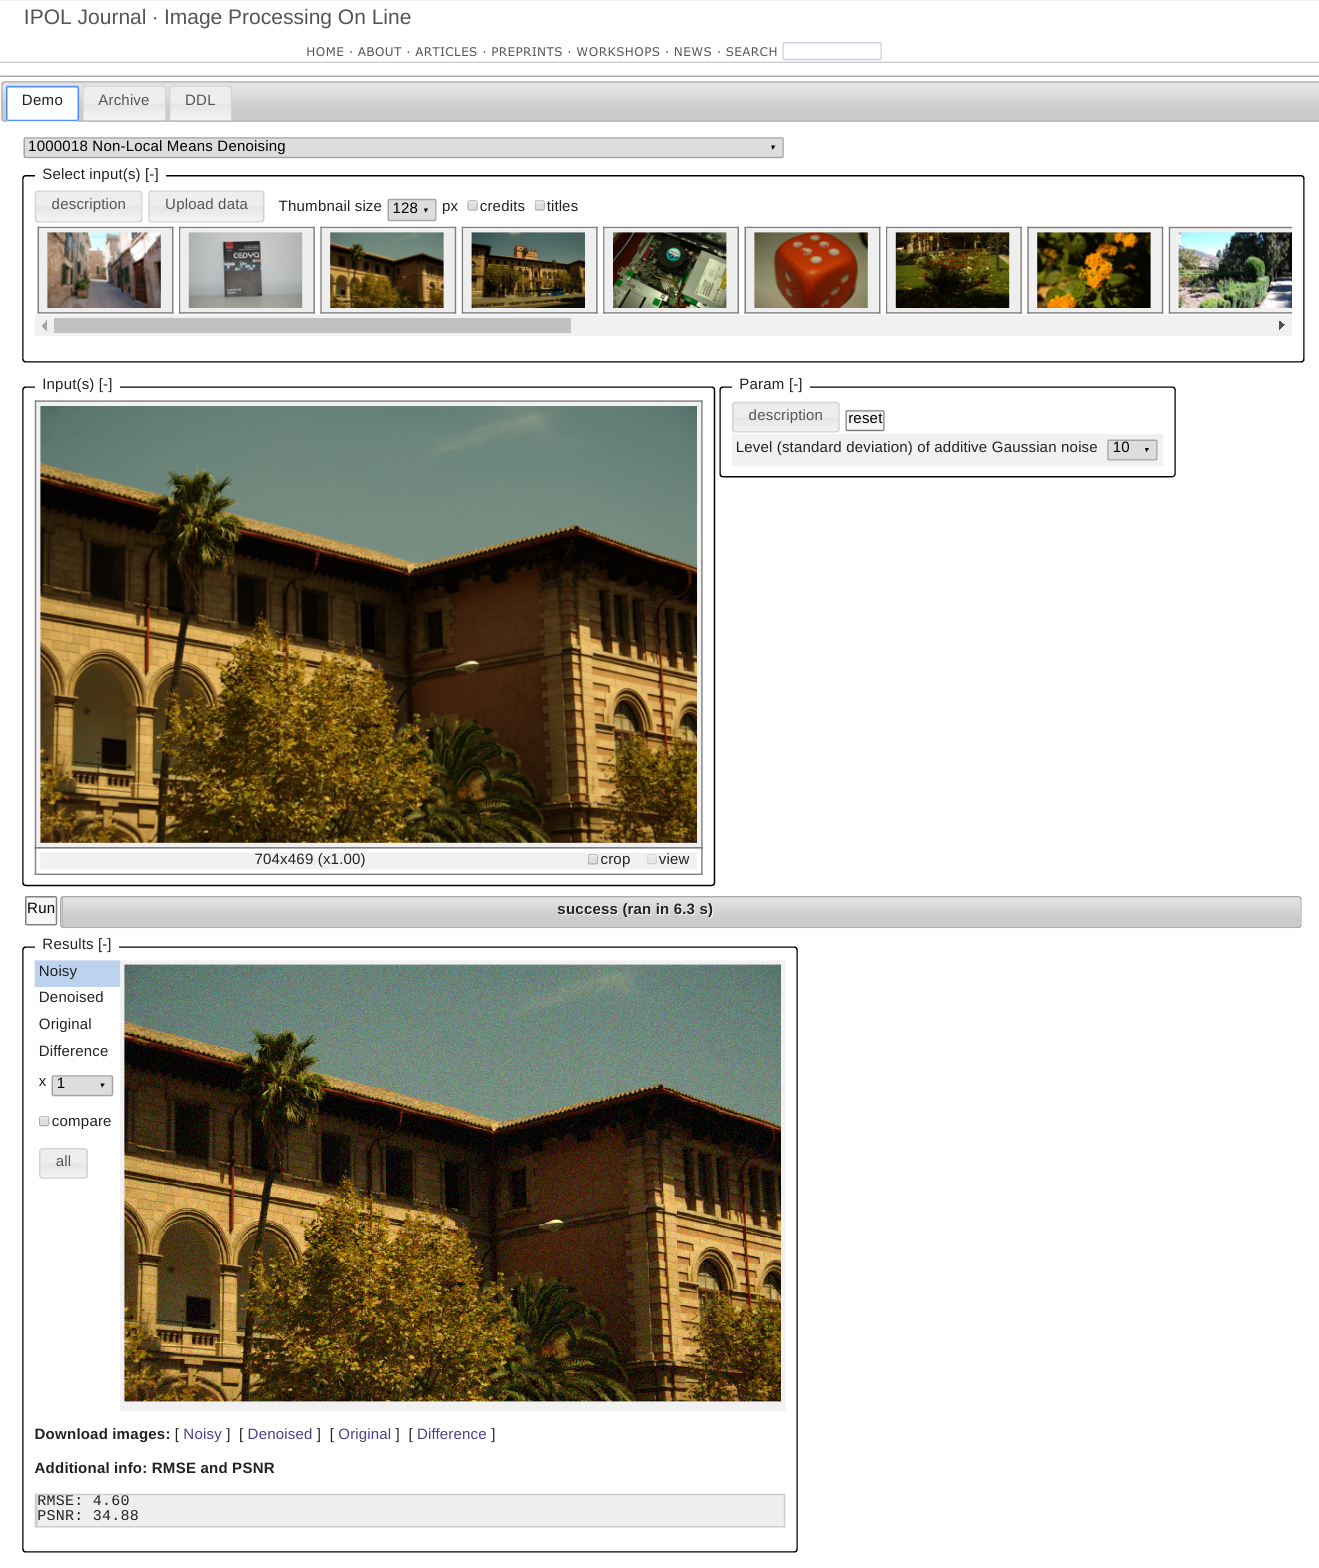
\includegraphics[width=3.5in]{Images/demo_snapshot}
  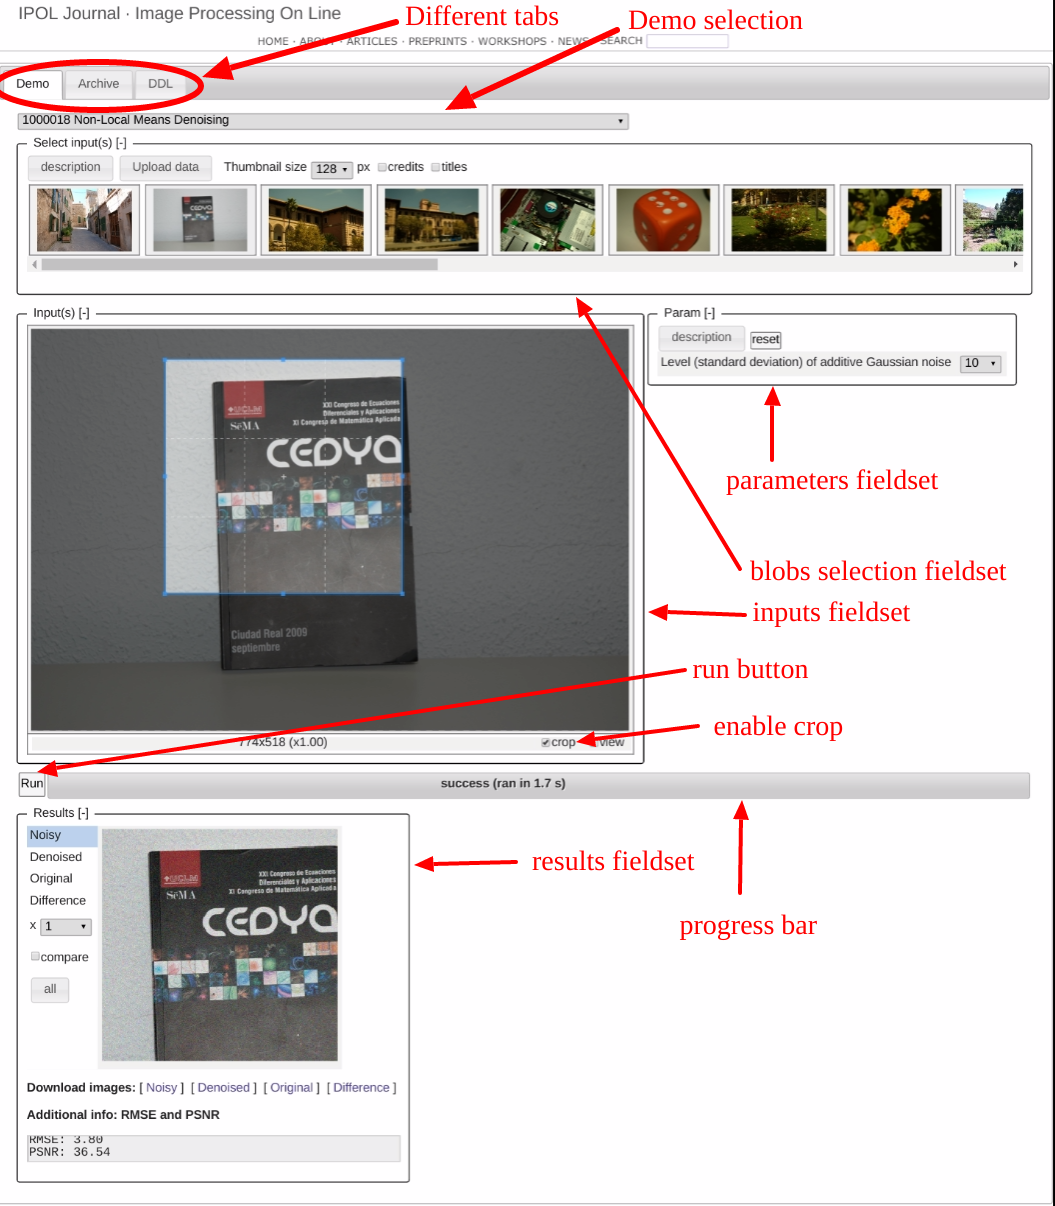
\includegraphics[width=3.5in]{Images/demo_capture}
  \caption{Demo display layout}
  \label{img:demo_snapshot}
\end{figure}

The main flow is as follows:
\begin{itemize}
 \item Step 1: select input demo
    \begin{itemize}
      \item read list of available demos and propose selection,
      \item or read demoid from url params
    \end{itemize}
 \item Step 2: Read and display list of available blobsets 
 \item Step 3: Select input blobset:
    \begin{itemize}
      \item select blobset from the list,
      \item or upload blobset.
    \end{itemize}
 \item Step 4: Display selected blobset 
    \begin{itemize}
      \item if there is a single image, allow crop selection,
      \item if there are several input blobs, show then in an ImageGallery object.
    \end{itemize}
 \item Step 5: Display the parameters and allow their selection. 
 \item Step 6: Allow 'run' button, on run click: 
    \begin{itemize}
      \item display progress bar,
      \item prepare the demo: check for compilation and installation of the source code,
      \item if blobset selection: send input blobset with possible crop,
      \item if blobset upload: crop input (if available) and send input blobset,
      \item execute the demo with the parameters.
    \end{itemize}
 \item Step 7: if upload, send results/parameters to archive. 
 \item Step 8: Display the results.
\end{itemize}

\subsubsection{Page template}

\paragraph{Included scripts and stylesheets}
The file "ipol\_demo.html" contains the page template, where the main displayed components are defined.
The different scripts are included, together with their CSS stylesheets:

\miguel{The LaTeX source was including directly JS code here from the sources by specifying actual line numbers, thus causing desynchronization and documentation outdating. The inclusion has been removed.}
%\lstinputlisting[language=HTML, , firstnumber=15, firstline=15, lastline=48, basicstyle=\scriptsize]{../../ipol_demo/modules/core/static/demo/clientApp/demo.html}

You will notice the use of the following external modules:
\begin{itemize}
 \item \emph{cropper.js} available at 
        \url{https://github.com/fengyuanchen/cropper} is used to crop input 
        images; 
 \item \emph{noUiSlider} available at 
        \url{http://refreshless.com/nouislider/} is used to create sliders that
        behave better on touch screen. It is combined with wNumb: 
        \url{http://refreshless.com/wnumb/} used to format outputs.
        Only basic features of noUiSlider are used for the moment, but more 
        advanced features could be added in the future, like displaying ticks 
        for example.
  \item In order to upload canvas images, the module 
        \emph{canvas-to-blob} 
        (\url{https://github.com/blueimp/JavaScript-Canvas-to-Blob}) and 
        \emph{blob-util} (\url{https://github.com/nolanlawson/blob-util}) are 
        used.
  \item \emph{sketch.js} is used for drawing mask, it has been 
        modified to better fit the needs of the mask drawing (and also to try 
        to fix a position issue with chrome on touching devices). The original   
        version is available at (\url{http://intridea.github.io/sketch.js/}), 
        the modified version is on the github server of the IPOL demo system.
  \item \emph{history.js} (\url{https://github.com/browserstate/history.js/}) is 
        used to push states on the browser history and to deal with  
        history events.
\end{itemize}

\paragraph{Page tabs} Three tabs are created using jquery ui, the first tab
contains the demo selection, display and execution. The second tab contains
the archive information, and the third tab contains the Demo Description 
Language (DDL) file in JSON format.
\miguel{The LaTeX source was including directly JS code here from the sources by specifying actual line numbers, thus causing desynchronization and documentation outdating. The inclusion has been removed.}
%\lstinputlisting[language=HTML, firstnumber=111, linerange={111-123}, basicstyle=\scriptsize]{../../ipol_demo/modules/core/static/demo/clientApp/demo.html}
$\cdots$
\miguel{The LaTeX source was including directly JS code here from the sources by specifying actual line numbers, thus causing desynchronization and documentation outdating. The inclusion has been removed.}
%\lstinputlisting[language=HTML, firstnumber=241,linerange={241-248}, basicstyle=\scriptsize]{../../ipol_demo/modules/core/static/demo/clientApp/demo.html}

Additionally, when the user enters the 'Archive' tab, the archive information
is automatically updated and the last archive page is displayed:
\miguel{The LaTeX source was including directly JS code here from the sources by specifying actual line numbers, thus causing desynchronization and documentation outdating. The inclusion has been removed.}
%\lstinputlisting[language=JavaScript, firstnumber=523,linerange={523-538}, basicstyle=\scriptsize]{../../ipol_demo/modules/core/static/demo/clientApp/demo.js}
To obtain the demo id, we first get the demo list stored within the "demo-select"
HTML element (using the jquery data() function), then we obtain the demo id 
(editordemoid) from the current position of the demo selection widget.

\paragraph{Page fieldsets and other displayed elements}

Four fieldsets are defined in the file ipol\_demo.html: blob selection, inputs, 
parameters and results. It also contains the code to create the progress bar
and the modal dialog to upload data.
The modal dialog is then initialized by the following code:
\miguel{The LaTeX source was including directly JS code here from the sources by specifying actual line numbers, thus causing desynchronization and documentation outdating. The inclusion has been removed.}
%\lstinputlisting[language=JavaScript, firstnumber=581,linerange={581-599}, basicstyle=\scriptsize]{../../ipol_demo/modules/core/static/demo/clientApp/demo.js}
and the ipol.upload.ManageLocalData() function called by ipol.setDemoPage().

\subsubsection{Step 1: input demo selection}

The list of demos is obtained from the demoinfo module using the service "demo\_list",
in the function ipol.ListDemos(). Once the list is obtained, 
ipol.OnDemoList(demolist) is called.
The demo list is stored in the HTML element "demo-select" and once the demo is
selected (from user selection or from the url parameters), the function 
ipol.setDemoPage() is called.

The function ipol.setDemoPage() first call the service "read\_last\-\_des\-crip\-tion\_from\_demo"
of the "demoinfo" module using ipol.utils.ModuleService():
\miguel{The LaTeX source was including directly JS code here from the sources by specifying actual line numbers, thus causing desynchronization and documentation outdating. The inclusion has been removed.}
%\lstinputlisting[language=JavaScript, firstnumber=317,linerange={317-321}, basicstyle=\scriptsize]{../../ipol_demo/modules/core/static/demo/clientApp/demo.js}

Once the demo description is returned, it runs the following steps:
\begin{itemize}
  \item empties the contents of the page,
  \item changes its title to contain the demo title,
  \item prepares the webpage to receive the different contents,
  \item displays the parameters if any,
  \item fills the contents of the archive tab,
  \item calls demoinfo module service "get\_blobs\-\_of\-\_demo\-\_by\-\_name\-\_ws"
to get the list of available blobsets for this demo, and calls staticOnDemoBlobs()
method to display them and set their events,
  \item and based on the "origin" parameter:
    \begin{itemize}
      \item if origin is "select\_widget" push a new state to the history,
      \item if origin is "url", if it contains the parameter 'res', displays
            the associated results. If it contains the parameter 'exp', displays
            the corresponding archive experiment.
      \item if origin is "browser\_history", call the callback function "func" 
            given in parameter.
    \end{itemize}
\end{itemize}

\subsubsection{Step 2: read and display list of available blobsets}

The static method ipol.DrawBlobs.staticOnDemoBlobs() returns a function
that creates an instance of ipol.DrawBlobs class, add possible template
to the blob list and displays all the blobs and their associated events.

\subsubsection{Step 3: select input blobset}

The input blobset can be either selected from the proposed list or uploaded from 
local files.
\paragraph{Blobset selection:}
If it is selected by clicking on one of the proposed blobsets, the event will
trigger the creation of a DrawInputs instance with the string "blobset" as origin,
load the input blobset and prepare for running the demo:
\miguel{The LaTeX source was including directly JS code here from the sources by specifying actual line numbers, thus causing desynchronization and documentation outdating. The inclusion has been removed.}
%\lstinputlisting[language=JavaScript, firstnumber=333,linerange={333-353}, basicstyle=\scriptsize]{../../ipol_demo/modules/core/static/demo/clientApp/ipol.drawblobs.js}

\paragraph{Data upload:}

Clicking on the "Upload data" button will display a modal dialog window
where the user can choose the files to upload from his local disk.
\begin{figure}[H]
  \centering
%  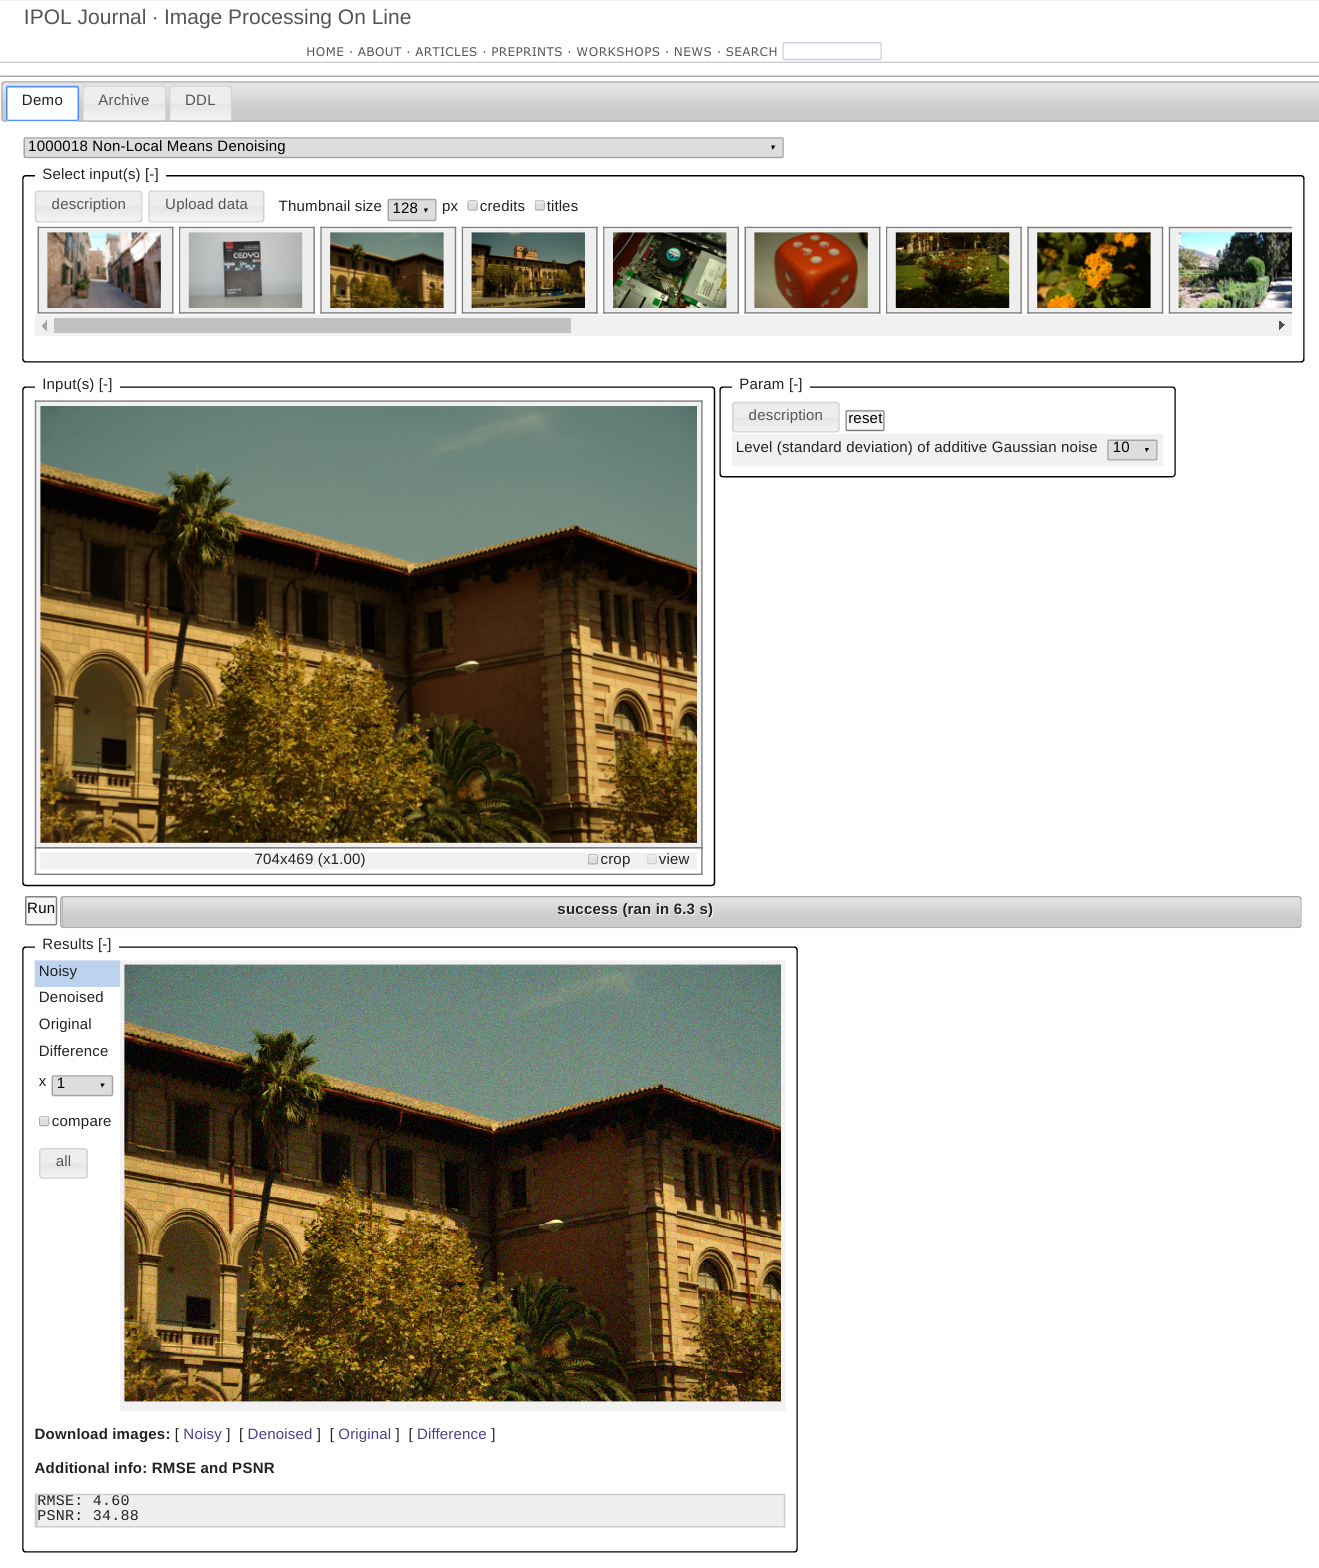
\includegraphics[width=3.5in]{Images/demo_snapshot}
  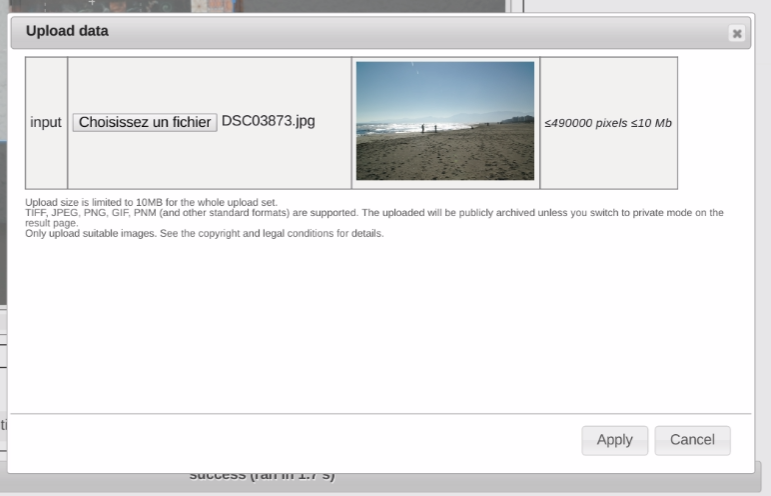
\includegraphics[width=3.5in]{Images/uploadwindow_capture}
  \caption{Upload files modal window}
  \label{img:uploadwindow_snapshot}
\end{figure}

This window is created by the ipol.upload.CreateUploadHTML(), and the function
ipol.upload.UploadBlobsEvents() deals with the file selection and display.
Note that the selected files will only be uploaded to the server before the
demo execution (after clicking on the "run" button).
Once the user accept its selection by clicking on the "Apply" button, 
instances of the DrawInputs and RunDemo classes are created within the 
ipol.upload.ManageLocalData() function:
\miguel{The LaTeX source was including directly JS code here from the sources by specifying actual line numbers, thus causing desynchronization and documentation outdating. The inclusion has been removed.}
%\lstinputlisting[language=JavaScript, firstnumber=160,linerange={160-185}, basicstyle=\scriptsize]{../../ipol_demo/modules/core/static/demo/clientApp/ipol.upload.js}

\subsubsection{Step 4: Display selected blobset}
Once the user has selected a blobset, it is displayed in the inputs fieldset
with its corresponding interface.
The initial HTML code is created by DrawInputs.createHTML() method. 

\paragraph{Single input image}
In the case of a single input image, this input is displayed with a crop option.
The user can crop the input image interactively and also display a zoomed preview
of the crop area on the right. The crop is using the existing "cropper.js" module.

\paragraph{Multiple inputs}
In the case of multiple inputs, the "ImageGallery" class is used to display the 
image representation of each input. In an input is of "image" type, it is its own
image representation. Otherwise, its image representation is a PNG image at the same
position in the blobset, if any.
The image gallery is created by the private method DrawInputs.\_createGallery(inputs\_info).
The "inputs\_info" object contains the titles and contents to be displayed and is created
by the one of the public methods DrawInputs.loadDataFromBlobset() or DrawInputs.loadDataFromLocalFiles().

\paragraph{Inpainting demos}
If the demo DDL has mask drawing enabled (general.drawmask=true), then an drawmask object
of class "ipol.features.Inpainting" is created as a private member \_drawmask of the class
DrawInputs. In this case, the usual displayed input is hidden and the displayed HTML code
contains the result of the function call to \_drawmask.createHTML() that creates all 
the mask drawing interface. The mask image is also added to the hidden ImageGallery object,
it will be updated after each drawing event and it will be used as an image to upload
for the demo execution.

\subsubsection{Step 5: Display the parameters and allow their selection}

The functions related to the display of the parameters are located in the "ipol.drawparams.js"
file and are within the class "ipol.DrawParams". Default parameter values can be reset using
the dedicated button.
The static method ipol.DrawParams.staticUpdateParams() takes care to updating parameters
that may have interdependencies. Currently, only the "visible" property type contents are 
evaluated using javascript eval() function.

\subsubsection{Step 6: deal with 'run' events}

The method "ipol.RunDemo.setRunEvent()" initializes the progress bar and deals
with the click on the "run" button.
The first step is to call the service "demorunner:init\_demo" that checks for the
source code installation and compilation. Once the current demo is successfully
initialized, input data can be either uploaded to defined:
\begin{itemize}
 \item for mask drawing demos, the method \_drawmask.submitDrawMask() is called,
        that will submit the inputs: image and mask.
 \item for non-mask-drawing demos where the input comes from a selected blobset,
        the service "demorunner:input\_select\_and\_crop" is called with all the
        required parameters: demo id, blobset information, crop information.
 \item for non-mask-drawing demos with local files to upload, a local variable
        of type "FormData" is instanciated and filled with the data to upload.
        In the case of a single input image with selected crop, the image
        is reduced to the crop area before its upload (using the getCroppedCanvas
        option of the cropper module). The convertion from canvas or img to 
        blobs that can be uploaded is obtained using either "canvas.toBlob()"
        function or "blobUtil.imgSrcToBlob().then()" function. Once the 
        form data is filled, the private method "\_uploadForm()" is called.
 \item for demos without any input blob, the private method "\_doRun()" is
        called in return of the service "demorunner:init\_noinputs".
\end{itemize}


%\bibliographystyle{plain}
%\bibliography{biblio}

\end{document}
% End of document



% Tests
\section{Tests}
\label{sec:Tests}
\subsection{Introduction}

The objective of the tests is to analyze automatically if the system fits the intended use. For that purpose the system is analized with two
types of tests, the first one are the Integration Tests in which individual software modules are combined and tested as a group, this implies from
the creation of a demo to its execution. The second one are the Unit Tests that are executed for each module and checks the response of all the
exposed methods.

Those tests are automatically executed in the integration and production enviroments every day by the crontab and every time a pull is made by 
the terminal.py script. If any of those test fail, an email is sent to all the emails listed in the /ci\_tests/send\_to.txt file.


\subsection{Integration Tests}

The integration tests are located in the /ci\_tests/system.py script and are responsible for testing all the IPOL modules and the interactions
between them. To accomplish that goal each test execute the full flow of the system, that goes from the creation of a demo, adding the DDL, blobs,
demoExtras, etc. to the execution of it.

Each test is independent from the others so the order in which it is executed is not important. To ensure that the state of the system has not been
altered by other test, the function setUp() is executed before every test. This function is responsible for cleaning the database from the 
remains of other tests.

\subsection{Unit Tests}

On each module there is a test.py script that executes all the unit test of the module. Each test check the correctness of every exposed method.

In the same way as the integration tests, each test can be executed in any order since the state of the system should not change after the execution
of the test.

\subsection{All.py}

This script is responsible for executing all the test, both the integration (system.py) and the unit test (test modules). To ensure
That several tests are not executed simultaneously, which could cause failures in the tests, a blocking system is implemented by the creation 
of the test.lock file, which if it exists implies that another instance of this script is running the tests.
If the script is blocked by this file it waits a random time between 5 and 10 seconds and check it again until it can run.


\subsection{Pull.sh}

This script is responsible for executing the git pull and call the all.py script to start all the tests. If any of the executed test fails an email
will be send to the email list reporting the failure.

This script is executed periodically every day at 10:00 am by the following instruction in the crontab: \begin{lstlisting}[language=Bash]
 0 10 * * * /home/ipol/ipolDevel/ci_tests/pull.sh
\end{lstlisting} in order to detect possible failures in the integration and production
enviroments, e.g. down modules, lack of disk memory, etc. Or every time a pull is made from the terminal.py script to check if the added cahnges do not
damage the system.


% Installation
\section{Installation of the project}


These are the steps that new members in the team need to follow to set up their environment.

\paragraph{General} \hspace{0pt} \\
\begin{itemize}
 \item Install Ubunto or Debian.
 \item Signup in Trello, Github and Slack.
 \item Add the new members emails to the servers list (PyLint and pdflatex) and Google Groups.
 \item Make the pull of the repositorie in GitHub.
  \begin{lstlisting}[language=Bash]
  ~/ipolDevel/git pull
  \end{lstlisting}
 \item Download a python IDE. e.g. Pycharm.
\end{itemize}

\paragraph{RSA} \hspace{0pt} \\
\begin{itemize}
 \item Create private/public keys.
  \begin{lstlisting}[language=Bash]
  ~/ssh-keygen
  \end{lstlisting}
\end{itemize}

\paragraph{SSH} \hspace{0pt} \\
\begin{itemize}
 \item Add your public key to the authorized\_keys file in the servers.
 \item Optional: Install the SSH server in your machine and add your public key to your own authorized\_keys to start the modules with the terminal.py.
\end{itemize}

\paragraph{Documentation} \hspace{0pt} \\
\begin{itemize}
 \item Download LaTex compiler. e.g. Kile.
 \item To be able to compile the documentation install texlive-full.
  \begin{lstlisting}[language=Bash]
  ~/sudo apt-get texlive-full
  \end{lstlisting}
 \item Generate all the pdfs of the documentation.
\end{itemize}

\paragraph{Libraries} \hspace{0pt} \\
\begin{itemize}
 \item Install all the python libraries with the follow command:
  \begin{lstlisting}[language=Bash]
  ~/pip install -r requirements.txt
  \end{lstlisting}
 \item Install all the libraries described in doc/system/ipol.pdf in the ``general\_notes'' section.
\end{itemize}

\paragraph{NGINX} \hspace{0pt} \\
\begin{itemize}
 \item Install nginx.
  \begin{lstlisting}[language=Bash]
  ~/sudo apt-get install nginx
  \end{lstlisting}
 \item Copy the config files that are in sysadmin/configs/nginx/default-local into the nginx folder /etc/nginx/sites-available/default and change the variable \$my\_user
\end{itemize}

\paragraph{Modules} \hspace{0pt} \\
\begin{itemize}
 \item Copy manually all the files that are not in the repo:
 
  \begin{itemize}
   \item ipol\_demo/modules/config\_common/authorized\_patterns.conf
   \item ipol\_demo/modules/config\_common/emails.conf
  \end{itemize}

 \item Copy from integration the DB and the staticData from demoinfo and blobs.
 \item Change the XML files in config\_common
\end{itemize}

\paragraph{CP} \hspace{0pt} \\
\begin{itemize}
 \item Add the hostname to the list ``local\_machines'' in the file ipol\_webapp/ipol\_webapp/ settings.py
 \item Follow the stepts described in ipol\_webapp/docs
 \item Create a new superuser in the local Control Panel
\end{itemize}

% General notes
\section{General notes}
In this section we add general comments on the projects, parts which still neeed to be written or coded. In general, information which needs to be documented but has not still found its place in the document. It works as a reminder not to forget.

\begin{itemize}
  \item The magic module. We use PIP, not the python-magic package found in most distributions. \ToDo{Explain why}.
  \item List of packages needed and how to install them.
  \item Description of the general requirements needed for a module to be part of the system (start, ping, and shutdown services ; structure of the general launching script...
\end{itemize}

- Example of another demo system: \url{http://places.csail.mit.edu/demo.html}

- Integrate Openseedragon, \url{https://openseadragon.github.io/}

- Document the format of the demo package, with desc.jon, images/, extra/, etc

- Most of our modules name the files according to the hash sum of their contents. This file names are OK for internal use, but the users should obtain the files with the proper names. This can be achieved with the ``download" attribute in HTML5. All website interfaces should provide the corresponding human-readable name. For example:

\begin{verbatim}
<a href="9021384984901238490128490123841222223312.png" download="denoised.png">
  Download the denoised image
</a>
\end{verbatim}

- Look for potential race conditions everywhere in the code, specially at the modules. Use locks to prevent them.

- All webservices should return a \emph{status:KO} when they fail. For example, if they're asked a service which doesn't exist they should return the status:KO, but never simply return a cherrypy message because of an untreated exception. Example of a wrong behavior:

\begin{verbatim}
http://ns3018037.ip-151-80-24.eu:9002/hello

404 Not Found

The path '/hello' was not found.

Traceback (most recent call last):
  File "/usr/lib/python2.7/dist-packages/cherrypy/_cprequest.py", line 670, in respond
    response.body = self.handler()
  File "/usr/lib/python2.7/dist-packages/cherrypy/lib/encoding.py", line 217, in __call__
    self.body = self.oldhandler(*args, **kwargs)
  File "/usr/lib/python2.7/dist-packages/cherrypy/_cperror.py", line 411, in __call__
    raise self
NotFound: (404, "The path '/hello' was not found.")
Powered by CherryPy 3.5.0
\end{verbatim}

- In general, check that no FK reference is missing at any of the database schemas of the modules, and that they're correct.
Also, we need to check absolutely that all the CASCADE DELETE are correct!

- FYI: the package \emph{sqlitebrowser} seems to be a very good tool to browse and develop the SQLite schemas.

- The demoInfo module returns \emph{Content-Type: text/html} instead of application/json:

\begin{verbatim}
curl --head http://ns3018037.ip-151-80-24.eu:9002/read_ddl?demodescriptionID=359
HTTP/1.1 200 OK
Date: Sun, 21 Feb 2016 19:41:29 GMT
Content-Length: 3545
Content-Type: text/html;charset=utf-8
Server: CherryPy/3.5.0
\end{verbatim}
\ToDo{Check that all modules return application/json and Content-Type: text/json;charset=utf-8}

Also, this module returns a JSON which contains a lots of backslashes!:

\begin{verbatim}
curl "http://ns3018037.ip-151-80-24.eu:9002/read_ddl?demodescriptionID=359"

{"status": "OK", "demo_description": "\"{\\\"archive\\\": {\\\"files\\\": {\\\"diffInputIHS.png\\\":
\\\"difference input-IHS\\\", \\\"diffInputPanS.png\\\": \\\"difference input-pansharpened\\\",
\\\"ihs.png\\\": \\\"IHS image\\\", \\\"input_0.sel.png\\\": \\\"input image\\\",
\\\"lowspectral.png\\\": \\\"lowspectral image\\\", \\\"pan.png\\\": \\\"pan image\\\",
\\\"pansharpened.png\\\": \\\"pansharpened image\\\"}, \\\"params\\\": [\\\"sfactor\\\"]},
\\\"build\\\": [{\\\"binaries\\\": [[\\\".\\\", \\\"pansharpening_ipol\\\"],
\end{verbatim}

This is clearly wrong. Compare with
\begin{verbatim}
curl "http://api.flickr.com/services/feeds/photos_public.gne?format=json"

sonFlickrFeed({
                "title": "Uploads from everyone",
                "link": "http://www.flickr.com/photos/",
                "description": "",
                "modified": "2016-02-21T19:58:40Z",
                "generator": "http://www.flickr.com/",
                "items": [
           {
                        "title": "P5302235",
                        "link": "http://www.flickr.com/photos/lievensoete/245457
53194/",
...
\end{verbatim}
\ToDo{Correct demoInfo so it returns a correct JSON response}

- A way to get images from the browser in a smartphone with HTML5: \url{http://don.github.io/html-cam/}

\ToDo{Keep adding!}


\section{To Do}
- Automatic testing. Two kind of tests:
\begin{itemize}
  \item For the IPOL system itself
  \item To ensure good compilation of the algorithm source codes
\end{itemize}

We can use PyUnit for the unit tests, but the most important is to have system-scope tests.

- Add statistics data collecting. Piwik can be used for this. Or Google Analytics, amongs others.


\bibliographystyle{plain}
\bibliography{biblio}

\end{document}
% End of document

